\documentclass[11pt]{article}
\usepackage[utf8]{inputenc}\usepackage[T1]{fontenc}\usepackage{lmodern}
\usepackage[margin=1in]{geometry}
\usepackage{microtype}\setlength{\emergencystretch}{3em}
\usepackage{amsmath,amssymb,booktabs,graphicx,array,xcolor,enumitem,caption}
\usepackage{longtable}
\graphicspath{{figures/}}
\usepackage[round]{natbib}
\usepackage[hidelinks]{hyperref}
% AUTO-GENERATED by paper/gen_results_macros.py. Do not edit by hand.
% Every value traces to a measured JSON artifact in this repository.
\makeatletter
\newcommand{\result}[1]{\@nameuse{result@#1}}
\makeatother
\expandafter\def\csname result@DebtOnlyDirect\endcsname{52}
\expandafter\def\csname result@DebtOnlyIndirect\endcsname{60}
\expandafter\def\csname result@AllClaimsDirect\endcsname{27}
\expandafter\def\csname result@AllClaimsIndirect\endcsname{47}
\expandafter\def\csname result@EquityShareDenom\endcsname{48}
\expandafter\def\csname result@DebtOnlyCV\endcsname{0.0506}
\expandafter\def\csname result@AllClaimsCV\endcsname{0.0942}
\expandafter\def\csname result@OneStepMovePct\endcsname{15}
\expandafter\def\csname result@SovereignUnion\endcsname{79}
\expandafter\def\csname result@SovereignCreditor\endcsname{32}
\expandafter\def\csname result@SovereignDebtor\endcsname{55}
\expandafter\def\csname result@GainsAGILow\endcsname{6.2}
\expandafter\def\csname result@GainsAGIHigh\endcsname{15.4}
\expandafter\def\csname result@ReceiptsShareLow\endcsname{0.6339}
\expandafter\def\csname result@ReceiptsShareHigh\endcsname{0.6528}
\expandafter\def\csname result@RetainedWageShare\endcsname{0.5683}
\expandafter\def\csname result@RequiredLow\endcsname{11.0}
\expandafter\def\csname result@RequiredHigh\endcsname{13.7}
\expandafter\def\csname result@TauKBarkai\endcsname{8.5}
\expandafter\def\csname result@TauKBarkaiLow\endcsname{7.3}
\expandafter\def\csname result@TauKBarkaiHigh\endcsname{9.9}
\expandafter\def\csname result@TauKKN\endcsname{1.5}
\expandafter\def\csname result@TauKPassLow\endcsname{0.1}
\expandafter\def\csname result@TauKPassHigh\endcsname{0}
\expandafter\def\csname result@TauKOperativeOld\endcsname{7.1}
\expandafter\def\csname result@ShareholderLayer\endcsname{0.0386}
\expandafter\def\csname result@ThetaTaxable\endcsname{27}
\expandafter\def\csname result@ThetaUntaxable\endcsname{73}
\expandafter\def\csname result@DeferralCentral\endcsname{0.601}
\expandafter\def\csname result@GainsUntaxedAtDeath\endcsname{46.9}
\expandafter\def\csname result@InterestSheltered\endcsname{32.8}
\expandafter\def\csname result@BondsRestOfWorld\endcsname{28.7}
\expandafter\def\csname result@BondsHouseholdDirect\endcsname{1.1}
\expandafter\def\csname result@FedCIT\endcsname{21}
\expandafter\def\csname result@FDDEIRate\endcsname{14.0}
\expandafter\def\csname result@CFCRate\endcsname{12.6}
\expandafter\def\csname result@RentBarkai\endcsname{0.351}
\expandafter\def\csname result@ShiftedShare\endcsname{48}
\expandafter\def\csname result@NInstitutions\endcsname{8,588}
\expandafter\def\csname result@NBanks\endcsname{4,296}
\expandafter\def\csname result@NCreditUnions\endcsname{4,292}
\expandafter\def\csname result@TopOnePctEquity\endcsname{50.9}
\expandafter\def\csname result@BottomHalfEquity\endcsname{0.6}
\expandafter\def\csname result@MPCWealth\endcsname{3.2}
   % measured values only

\newif\ifanon
\ifdefined\ANON\anontrue\else\anonfalse\fi

\title{\bfseries Wage Risk Is Sovereign Risk: Labor Backing Accounts\\ and AI Exposure}

\ifanon
  \author{\normalsize\itshape Author names and affiliations removed for double-anonymous peer review}
\else
  \author{%
    Mohit Pratap Singh Rathore\thanks{Oviqo. Corresponding author.}\quad
    Gunveer Singh Kalsi\thanks{Oviqo.}\quad
    Sriharsha Meduri\thanks{Oviqo.}\quad
    Pratap Chandra Mandal\thanks{Indian Institute of Management Shillong.}}
\fi
\date{}

\begin{document}
\maketitle

\begin{abstract}
\noindent
We introduce labor backing accounts, a decomposition of United States financial claims by the
income that services each claim and by who holds, guarantees or owes it. About
\result{DebtOnlyDirect} percent of all US debt, public and private, is serviced directly from
wages, and \result{DebtOnlyIndirect} percent once indirect servicing is counted; government debt
enters through the labor-linked share of the receipts that service it, not because a household
owes it. The holder map shows an asymmetry: the federal government is exposed, as holder,
guarantor or debtor, on about \result{SovereignUnion} percent of directly wage-backed claims and
on about \result{AIFederalShareRounded} percent of the claims on artificial intelligence capital.
Rebuilding the effective marginal rate on income that shifts from wages to AI capital, every layer
of tax counted once, gives \result{TauKBarkai} percent against the \result{RequiredEasy} to
\result{RequiredHard} percent needed to replace the wage taxes lost. It falls short on both
defensible bases for the share of equity the income tax reaches. At the one displacement level
inside our data the loss is overwhelmingly fiscal rather than financial. The state loses in both directions through different tax bases, so one
capital tax rate is asked to do two opposite jobs.
\end{abstract}

\vspace{0.5em}
\noindent\textbf{Keywords:} fiscal exposure; automation; labor share; capital taxation;
sovereign risk; financial claims

\section{Introduction}
\label{sec:intro}

A government that guarantees mortgages, lends for education and funds itself from payroll and
income taxes has taken a position on wages without ever describing it as one. If automation moves
income from labor to capital, that position loses value on both sides at once: the revenue that
services the debt falls, and the credit the government has guaranteed deteriorates for the same
reason. Whether it holds an offsetting claim on the capital that replaced the labor is an
empirical question, and it is the question this paper answers.

The answer is that it does not. Measured on the same basis and in the same period, the United
States holds the wage side of a two-sided bet on artificial intelligence and almost none of the
other side. That is a structural observation about who holds what, not a forecast about which
direction events will take, and it has a consequence in both directions: if AI succeeds and
displaces labor, wage taxes fall and wage-backed credit deteriorates; if AI disappoints, capital
gains and corporate receipts fall instead. The federal government loses in both cases, through
different tax bases, and in neither does it hold a claim large enough to offset the loss.

Three measurements carry the argument. About \result{DebtOnlyDirect} percent of all US debt,
public and private, is serviced directly from wages, and \result{DebtOnlyIndirect} percent once
indirect servicing is counted. The federal government is exposed, as holder, guarantor or debtor,
on about \result{SovereignUnion} percent of those directly wage-backed claims, against about
\result{AIFederalShareRounded} percent of the claims on AI capital. And income that moves from
wages to AI capital bears an effective marginal tax rate of about \result{TauKBarkai} percent,
where replacing the wage taxes lost would require \result{RequiredEasy} to \result{RequiredHard}
percent.

\paragraph{Contributions.} The paper makes four.

\begin{enumerate}[leftmargin=1.4em,itemsep=0.25em]
\item \textbf{A measurement framework.} Labor backing accounts decompose the whole stock of US
financial claims two ways at once, by the income that services each claim and by who ultimately
holds, guarantees or owes it. The framework yields a ratio, a federal exposure share, a holder map
for both sides of the exposure, a series running from 1952, and a breakdown by wage quintile. The
construction, the conventions, and the sensitivity of each result to the judgement calls behind it
are stated in full, including the one convention that does most of the work.

\item \textbf{A holder map that shows the asymmetry.} The wage side and the AI side are measured
on the same basis so that the two can be compared rather than asserted. The AI side is built from
on-balance-sheet filings alone, so it is a lower bound and the federal share of it an upper bound,
which means the asymmetry we report is the conservative version of it.

\item \textbf{An explanation of why the tax system cannot close the gap.} We rebuild the effective
marginal rate on income that shifts from wages to AI capital from components, taking the treatment
of expensing from \citet{AcemogluManeraRestrepo2020} rather than assuming it, and show that the
binding constraint is the ownership of corporate claims rather than offshore profit shifting.
About \result{ThetaUntaxable} percent of US corporate equity is held in forms the individual
income tax barely reaches, and about \result{GainsUntaxedAtDeath} percent of accrued gains are
never taxed because basis is stepped up at death.

\item \textbf{A measured incidence of displacement.} At the only displacement level inside the
observed data we measure where the first-round loss lands across the federal government,
households, the housing agencies and \result{NInstitutions} bank and credit union balance sheets,
and we test whether household relief protects bank capital. It does not, and the reason it does
not is measured rather than argued.
\end{enumerate}

\paragraph{What we do not claim.} We do not forecast the pace of automation, and we do not claim
that AI will displace any particular quantity of labor: the paper reports a response surface
rather than a point on it. Only one level, ten percent of the wage bill, sits inside the range of
the data used to calibrate reemployment; every figure above that is labelled scenario and reported
as a band. We do not claim the fiscal mechanism, which is established in the literature reviewed
in Section~\ref{sec:related} and which we take as our starting point rather than our finding. We
do not claim that the measurement framework is new in the strong sense: our search located no
prior construction of the same object, but that search was not systematic, so the claim is stated
as ``none located'' rather than ``none exists''. And we do not claim that the capital tax result
settles which tax base is the right one; we argue for a marginal, flow-based rate and state the
case against it plainly in Section~\ref{sec:fiscal}.

\paragraph{Research questions and objectives.} RQ1 asks what share of US financial claims is
serviced by labor income, and who holds those claims; RO1 constructs the labor backing accounts
and the holder map, in Section~\ref{sec:accounts}. RQ2 asks whether the capital tax system can
replace the revenue lost when income shifts from wages to AI capital; RO2 builds the effective
rate from components and compares it with the required rate, in Section~\ref{sec:fiscal}. RQ3 asks
where the loss from displacement lands, by holder; RO3 measures first-round incidence at the level
inside the data, in Section~\ref{sec:displacement}. RQ4 asks what the second round does to the
institutions that hold the credit, and whether household relief protects them; RO4 applies the
losses across individual balance sheets, in Section~\ref{sec:banks}. RQ5 asks what happens in the
opposite direction, if AI disappoints; RO5 prices that case on the same basis, in
Section~\ref{sec:bust}. RQ6 asks what follows for institutions; RO6 sets out the minimum
sufficient set of instruments at each regime, and what the evidence does not support, in
Section~\ref{sec:institutions}.

\paragraph{How to read the numbers.} Every quantitative statement in this paper carries a status
on its first use. \emph{Replicated} means rebuilt by an instance that did not write the code, from
raw data and a published brief alone, inside a tolerance stated before the rebuild.
\emph{Measured} means produced by the pipeline and clearing every applicable check, but not
independently rebuilt. \emph{Scenario} means arithmetic conditional on an assumption stated where
the number appears. Quantities that were withdrawn appear only in Section~\ref{sec:limitations},
which lists them with reasons. Every number in the text is generated from an artifact in the
replication package rather than typed, and the same artifacts generate the tables.


\section{Related work}
\label{sec:related}

This paper sits in a literature that has established most of its framing, and the honest way to
position it is to say what each neighbouring work did before saying what is left. We group the
work by theme and end the section with the boundary stated exactly.

\subsection{AI and the public finances}

The proposition that labor-displacing AI is a fiscal event before it is anything else is
established, and this paper does not claim it.

\citet{PriceSuresh2026} measure it directly. Working in a budget model, they put about
eighty-four percent of federal revenue on individual or payroll taxes and roughly two thirds of it
directly on labor, and run four AI substitution scenarios on two axes, one of which is the
reemployment rate and the other the pricing of AI services. Those are the same two quantities this
paper calls the retained wage share and the effective rate on AI capital. Their policy options are
explicitly illustrative and unsized. Because output is held constant by construction, their
exercise is the analogue of our output-preserved case alone, and it carries no household debt, no
mortgages and no bank balance sheets.

\citet{Barhoumi2026} is a workshop synthesis rather than a model, and it contains no numbers; what
matters for our purposes is that it states the mechanism this paper measures. It says directly
that large-scale job losses weaken household balance sheets and raise default risks in banking
systems exposed to consumer credit, and it states the distributional asymmetry, that the costs
fall on incumbent workers and borrowers while the gains accrue to new entrants and AI-intensive
firms. Both sides of the exposure appear in the same paragraph of that note. What is absent is any
measurement of them, and any map of who holds them. It is the closest approach to this paper's
question that we located, and we say so rather than leaving a reader to find it.

\citet{IeongSaputraManiarCheng2026} build a four-channel account of how a labor-displacing
transition erodes a tax base, simulated for an average OECD country: the shift from
highly-taxed labor income to lower-taxed capital income, leakage when AI providers are
non-resident, consumer benefits that are never taxed, and higher social support spending. The
first channel is the fiscal condition of Section~\ref{sec:fiscal} stated in a different accounting
frame. The scenarios in the workshop synthesis above were developed in collaboration with this
group, which connects two works that might otherwise look independent, and we treat all three as
connected work rather than as competition.

\citet{KorinekLockwood2026} ask the optimal-taxation question across stages of an AI transition.
That is a different question from ours. We measure what the existing tax system does reach; they
characterise what an optimal one should do. \citet{FalkTsoukalas2026} make an argument that is
stronger than ours and reaches it first: each firm captures the full cost saving from automation
while bearing only a fraction of the demand loss it creates, so capital income taxes cannot
resolve the externality and a Pigouvian automation tax is the instrument that can. Our
contribution here is not the verdict but the calibration, and our measured effective rate can be
read as an input to their argument rather than a competitor to it.
\citet{CasasTorres2024} established the base-shift mechanism two years before this project began,
showing in general equilibrium that as automation rises the ratio of fiscal revenue to output
falls, because the inputs that bear the tax are replaced by an input that does not.
\citet{Brollo2024} supplies the one measured policy effect we rely on in
Section~\ref{sec:institutions}, that more generous unemployment insurance substantially attenuates
the wage decline from robotisation.

\paragraph{What this paper does differently.} None of these decomposes the stock of financial
claims by the income that services it, and none records who holds each side. They establish that
the revenue falls. We measure whose balance sheets the claims sit on when it does.

\subsection{Automation, labor demand and reemployment}

\citet{AcemogluRestrepo2020} is the empirical anchor for what displacement does to employment and
wages, and the source of the reemployment structure our retained wage share is built on.
\citet{AcemogluManeraRestrepo2020} does double duty here. It supplies the tax result that
Section~\ref{sec:fiscal} takes as derived rather than assumed, that under full expensing the
normal return is relieved at the entity level so the marginal rate on it is the owner's rate
alone, and it is the source of the observation that the US tax system taxes capital more lightly
than labor at the margin. \citet{Huckfeldt2022} gives the wage loss on reemployment that our
retained wage share uses, and the finding that the loss is concentrated among occupation switchers
rather than spread evenly.

\citet{ManningAguirreMuroMethkupally2026} build an occupation-level index of adaptive capacity and
find, against what one might expect, that AI exposure and adaptive capacity are positively
correlated: most workers in the most exposed occupations are in occupations with above-median
capacity to absorb a transition. That is the same conclusion this paper reaches from household
microdata in Section~\ref{sec:displacement}, on a different object: exposure alone does not
identify vulnerability, and pay does most of the work.

\paragraph{What this paper does differently.} An occupation-level index cannot show that the
relationship between buffers and exposure runs through pay level and disappears once pay is
controlled, because that is a household-level result requiring household balances. Nor can it
show that the thinnest buffers sit in the second wage quintile rather than the first.

\subsection{Capital taxation and the ownership of corporate claims}

Our effective rate is assembled from a literature that has measured its components separately.
\citet{Auerbach2017} sets out the structure of taxing the corporate return and the sense in which
expensing exempts the normal return. \citet{Barkai2020} supplies one of the two rent share
readings we carry, and the incompatibility between that reading and its main alternative is why we
report both and never average them. \citet{TorslovWierZucman2023} supplies the profit-shifting
share, which we report because it matters and rank fourth among seven levers because it does not
matter most. The ownership parameters that turn out to be decisive, the share of corporate equity
in taxable accounts, the deferral of tax between accrual and realization, the share of gains never
taxed because basis is stepped up at death, and the tax status of corporate debt, come from work
in the public finance and budget-office literature that we cite at the point of use.

\paragraph{What this paper does differently.} These components have not, so far as we located,
been assembled into a single marginal effective rate on the income that moves from wages to AI
capital, and compared against the rate that revenue replacement would require. The assembly is
where the ownership explanation becomes visible: the reason the rate is low is who owns the
claims, not where the profits are booked.

\subsection{Household balance sheets, default and stress testing}

The household side of this paper rests on a literature about what job loss does to a borrower.
\citet{BhuttaBrickerDettlingKelliherLaufer2019} and \citet{MerikullRoom2020} establish the
relationship between income shocks, liquid buffers and distress that our engine's uplifts rely on,
and \citet{AlbaceteFessler2010} is the stress-testing template our engine follows in structure. Our
own default uplifts are taken from the literature on job loss and mortgage default rather than
estimated here. \citet{CohenKillenLau2026} supplies the measured size of bank commitments to
AI-adjacent industries that Section~\ref{sec:bust} uses, and is the one source in this paper that
sits on both sides of the exposure at once.

\citet{Chen2026} is the largest overlap with this paper, and it is with our second round. It is a
macro-financial stress test of rapid AI adoption with eleven testable predictions, reaching private
credit and mortgages, and it makes the point that AI exposure is concentrated among high-income
households who account for a large share of consumption. What remains ours is severity measured
against a named supervisory benchmark, loss rates by loan category, application across individual
balance sheets, and the decomposition of the loss by holder.

\paragraph{The closest existing statistic.} The Federal Reserve's debt service ratio measures
household debt service against all household income, and the distributional financial accounts
give balance sheets by wealth percentile. Both are closer to our object than anything else
published. Neither decomposes the servicing cash flow by the income that supplies it, and neither
extends beyond households to the rest of the claim structure.

\subsection{What is ours}

\begin{quote}
The fiscal mechanism is established. What this paper adds is the measured holder structure of the
claims that wages pay, on both sides of the exposure and on the same basis; household losses from
survey microdata mapped to the supervisor's own loss rates; the incidence of those losses by who
bears them; a capital tax condition assembled from sourced components and independently rebuilt;
and a public claims register in which every reported quantity carries its status and its
replication flag.
\end{quote}

One boundary statement belongs here rather than in the limitations, because it qualifies the
contribution rather than the result. Our search located no prior construction of the labor backing
accounts as an object. That search was not systematic, so the claim we make is ``none located''
rather than ``none exists''. We have already retired one priority claim in this project after a
non-systematic search found prior work, and the same could happen here.


\section{Data and method}
\label{sec:data}

This section states what each module is built from, what it holds fixed, and how a reader should
weigh what comes out of it. It supports every later section, and it sets the vocabulary used to
label results.

\paragraph{What the displacement engine is.} It is a conditional labor-income-loss stress test. A
share of the wage bill is removed by assumption, and the engine reports what follows for the
budget, for household credit and for individual balance sheets. It contains no model of
artificial intelligence, no adoption path and no forecast. Every displacement figure in this
paper is therefore conditional balance-sheet arithmetic, not a causal estimate and not a
prediction, and the level is an input rather than a result.

One level, ten percent of the wage bill, is reported throughout as the case with the least
extrapolation, and that phrase is meant literally rather than as a claim to observation. What
stays inside its observed range there is the reemployment relationship. The default uplifts are
transferred from a different episode, the allocation of displacement across households is assumed,
and the transmission from lost income to spending is a stated mapping. So the ten percent case is
a calibrated scenario whose weakest link is calibrated to data, not an observed or causally
identified result.

\subsection{Sources}

Claim levels and holder shares come from the Federal Reserve's financial accounts
\citep{FRBZ1}, read from the published data package. The instrument suffix in that release is not
the same across sectors, so bank, insurer and central bank holdings of one instrument sit under
different codes; matching on the exact suffix pushes whole holder classes into an unallocated
remainder. We match on the instrument family and take the closest suffix per sector, which cuts
the aggregate remainder from about a fifth to under two percent. Every series used is recorded
with the publisher's own description in the replication package.

Household balances come from the Survey of Income and Program Participation \citep{CensusSIPP},
household composition, earnings and occupation from the American Community Survey
\citep{CensusACS}, and official credit aggregates from the New York Federal Reserve
\citep{NYFedHHDC2026}. The wage share of adjusted gross income, and the realized gains bound that
travels with it, are from the Statistics of Income \citep{IRSSOI}; reemployment is fitted on
fourteen biennial vintages of the worker displacement release \citep{BLSWorkerDisplacement}; loss
rates and scenario severities are from the supervisory stress test \citep{FRBDFAST2026}; trust
fund income and depletion dates from the trustees' report \citep{SSATrustees2026}; the
distribution of corporate equity from the distributional financial accounts \citep{FRBDFA} and
behind them the Survey of Consumer Finances \citep{FRBSCF}; and the housing agency book from the
Enterprises' annual filings \citep{FannieMae10K2025,FreddieMac10K2025}. The AI side is built from
the filings of nine registrants, with the off-balance-sheet structures described by
\citet{BIS2026} absent from them. The wage bill and federal receipts used as bases are
\result{WageBillBn} and \result{FedReceiptsBn} billion dollars. Units are taken from the provider
at retrieval rather than assumed, and a discontinued series is replaced rather than carried.

\subsection{The household credit engine}

The engine maps a displacement level onto household credit losses without naming a set of
displaced households. Displacement is a probability applied to every household in the working
core, defined as a household with at least one employed member aged 25 to 64. The share of
earners displaced is set equal to the share of the wage bill displaced, and each household's
earners are drawn against that share.

A household that loses an earner does not default; it becomes more likely to default. The
uplift is five percentage points for one displaced earner and eight for two
\citep{GerardiHerkenhoffOhanianWillen2018}, and losses are exposure at default times loss given
default, with severities of 0.25 to 0.40 on first-lien mortgages, 0.80 to 1.00 on cards, 0.45 to
0.65 on auto and 0.75 to 1.00 on student debt. Applying a portfolio loss rate to exposure at
default instead would count the probability of default twice.

Survey balances are benchmarked to official aggregates first, and two ratios do different work.
The \emph{under-reporting factor} is the official aggregate over the full survey universe and is a
survey correction; the \emph{coverage share} is the working-core balance over that universe and is
a fact about which households the analysis covers. Table~\ref{tab:underreporting} gives both. The
identity between them holds to three decimals on every book, and all four factors were rebuilt
independently.

\begin{table}[htbp]
\centering
\caption{Survey balances benchmarked to official aggregates, 2026:Q2. The under-reporting factor
corrects the survey; the coverage share describes the analysis sample. Rebuilt.}
\label{tab:underreporting}
\setlength{\tabcolsep}{4pt}
\begin{tabular}{lrrrr}
\toprule
Book & Official aggregate (USD bn) & Survey universe (USD bn) & Under-reporting factor & Coverage share \\
\midrule
Mortgage & 13,100.0 & 10,403.3 & 1.2592 & 0.8205 \\
Credit card & 1,357.2 & 539.5 & 2.5159 & 0.7400 \\
Auto & 1,713.0 & 899.9 & 1.9036 & 0.7737 \\
Student & 1,650.0 & 1,159.3 & 1.4233 & 0.8832 \\
\bottomrule
\end{tabular}

\end{table}

One scope statement travels with every credit number here. The engine is first round only: house
prices, consumer spending, business revenue and the employment of everyone not displaced are held
fixed. Against a supervisory scenario, which moves all of those together, the figures are a lower
bound rather than an estimate.

\subsection{The fiscal module and the second round}

The fiscal module converts displacement into a dollar amount against the wage bill and applies a
loss per dollar with three parts: the labor tax no longer collected on wages that are not
re-earned, less the capital tax collected on the income that displaced them, plus any outlay
response. The share of wages re-earned is governed by a reemployment rate fitted on the
displacement vintages against labor market slack and solved as a fixed point, since displacement
changes the slack the fit is a function of. Losses are reported for the terminal year rather than
as a cumulative total divided by a horizon, and they are not linear in displacement: the share
re-earned falls as displacement rises. Trust fund effects use each fund's own payroll share of its
own income.

The second round is the weakest module evidentially and is labeled scenario wherever it appears.
The net fall in wage income becomes a demand shortfall through the difference between the
propensity to consume out of labor and out of capital income
\citep{MianStraubSufi2020,FagerengHolmNatvik2021}; the shortfall is expressed as a share of output
and compared with the fall in output in the supervisory severely adverse scenario; and the
supervisor's own published loss totals are scaled by that ratio. House prices enter through an
income elasticity \citep{HarterDreiman2004}, and employment through an Okun coefficient
\citep{BallLeighLoungani2017}. Three elements have no source: the shape of the loss curve beyond
the supervisory point, for which we carry a linear, a capped and a convex mapping; the propensity
ranges, measured on transitory shocks where displacement is persistent; and the path itself. We
report the whole grid of 648 combinations as a band and never a point inside it.

\subsection{Institution-level data}

The second round is applied across individual balance sheets rather than to an aggregate. The
panel is every insured bank and credit union at 30 June 2026, with the loan book by category and
the capital measure each is tested against: the tier 1 leverage ratio against its four percent
threshold for banks, the net worth ratio against its six percent threshold for credit unions.
After exclusions it is \result{NInstitutions} institutions, \result{NBanks} banks and
\result{NCreditUnions} credit unions, holding \result{SystemAssetsBn} billion dollars of assets.

\result{ExcludedInstitutions} institutions holding \result{ExcludedAssetsBn} billion dollars are
excluded because they report neither tier 1 capital nor total equity, being overwhelmingly insured
US branches of foreign chartered institutions whose capital sits at the parent; a capital test
shows them breaching before any loss, which is an artifact of a missing field. A capital test is
only informative if almost nothing fails it before any loss, and after the exclusion
\result{BaselineBreaches} institutions breach at baseline, \result{BaselinePctAssets} percent of
system assets. Losses are allocated pro rata by category holdings, so dispersion reflects business
mix alone and is a lower bound on true dispersion.

\subsection{Status labels, and what was independently rebuilt}
\label{sec:rebuild}

Three labels are used throughout and appear in every table caption. \emph{Rebuilt} means the
quantity was reproduced by an independent computational rebuild: a separate run that had no access
to this project's code and worked from raw data and a published specification alone, inside a
tolerance fixed before the rebuild began. \emph{Measured} means produced by the pipeline, clearing
every applicable bounds check, but not independently rebuilt. \emph{Scenario} means arithmetic
conditional on an assumption stated where the number appears. In prose we give the label where a
reader could otherwise mistake a scenario for a measurement; elsewhere the table caption carries
it.

What a rebuild establishes needs saying plainly, because the word invites more than it should. It
establishes computational reproducibility: that the stated inputs and the stated construction
produce the stated number. It says nothing about whether the construction is the right one, or
whether the economic assumptions behind it hold. A quantity can be rebuilt to six decimal places
and still rest on an assumption we have no evidence for, and several in this paper do.

Three rebuild rounds have been run. Round two scored \result{RepTwoScored} quantities,
\result{RepTwoSealed} of them against expected values fixed in advance;
\result{RepTwoFivePct} came within five percent and \result{RepTwoTolerance} inside the stated
tolerance, and \result{RepTwoMismatch} did not match. Round three covered the two constructions
the earlier rounds had not reached, the debt-only ratio and the assembled capital tax rate, and
matched all \result{RepThreeSealed} quantities, \result{RepThreeRounding} of them within
rounding. The blind was procedural rather than enforced: the rebuild ran on the same machine, with
the file of expected values reachable at a path the specification names, and reported it unopened
until the rebuild was final. The claim is therefore that these quantities were independently
rebuilt under a reported blind protocol, not that they were independently verified.
Appendix~\ref{app:rebuild} gives the round-by-round detail and the causes of the mismatches.

Separately, a standing bounds check states the bound a quantity must respect before it is
computed and tests it afterwards, running \result{PlausChecks} checks with
\result{PlausViolations} violations, all of them superseded rows retained deliberately.

\subsection{Disclosure of AI assistance}
\label{sec:aidisclosure}

The conceptual model, the definitions, the inclusion and exclusion rules, the equations, the
scenario definitions, the statistical choices and the interpretation of results are the authors'.
Generative AI tools provided computational assistance, in writing and checking analysis code, and
drafting assistance with the text; the independent computational rebuilds were carried out by
separate instances of such tools working from published specifications. The authors reviewed every
output and take responsibility for the content. No reported value originates in a model's
assertion: every number in the text and tables is generated from a measured artifact in the
replication package.


\section{Labor backing accounts}
\label{sec:accounts}

This section sets out the paper's method contribution. Labor backing accounts decompose the
whole stock of United States financial claims twice over: once by the income that services each
claim, and once by who ultimately holds, guarantees or owes it. The two decompositions are taken
on the same claim stock in the same period, which is what allows the wage side and the AI side of
the exposure to be compared rather than asserted. Everything later in the paper is built on the
object defined here.

\subsection{Definition and vocabulary}

A financial claim is serviced out of some income stream. A mortgage is serviced out of household
wages; a corporate bond out of business revenue; Treasury debt out of federal receipts, which are
themselves drawn from wages, from capital income and from other sources in measurable
proportions. The \emph{labor backing} of a class of claims is the share of the cash flow that
services it which is labor income. A claim is \emph{directly wage-backed} when wages pay it
without passing through another party's income statement first. It is \emph{indirectly
wage-backed} when wages first become spending, spending becomes business revenue, and that
revenue services the claim.

The distinction is the accounting form of one the rest of the paper uses throughout. The
\emph{first round} is what happens to the party whose own wages fall. The \emph{second round} is
what happens to everyone else, through the spending, house prices and business credit that
follow. Direct backing is the first round seen on the liability side of the economy; indirect
backing is the second.

Two conventions of presentation travel with every result below. \emph{Displacement} is always
stated as a share of the total wage bill, never as a count of jobs and never as a share of one
occupation, because the fiscal and the credit channel both run on dollars of pay. And every
quantitative statement carries a status on its first use. A \emph{replicated} figure was rebuilt
by an instance that had not written the code, from raw data and a published brief alone, inside a
stated tolerance. A \emph{measured} figure comes from the pipeline and clears every applicable
check but has not been independently rebuilt. A \emph{scenario} figure is arithmetic conditional
on a stated assumption. Section~\ref{sec:data} sets out how the labels are assigned and what they
are worth.

The accounts run over thirteen classes of claim drawn from the Federal Reserve financial
accounts, listed with their levels in Table~\ref{tab:classes}. They cover household mortgage and
consumer credit, multifamily and commercial mortgages, Treasury and state and local debt,
corporate bonds and loans, noncorporate business debt, and corporate equity.

\begin{table}[htbp]
\centering
\caption{The thirteen claim classes, levels and labor backing, 2025. Classes marked $\dagger$ are
serviced from business revenue and carry zero direct backing under the one-step rule. Measured;
the home mortgage and multifamily coefficients are replicated.}
\label{tab:classes}
\begin{tabular}{lrrr}
\toprule
Claim class & Level (USD bn) & Labor backing & Wage-backed (USD bn) \\
\midrule
Home mortgage & 13,788.3 & 0.8104 & 11,173.5 \\
Credit card & 1,324.3 & 0.7302 & 967.0 \\
Auto loan & 1,562.2 & 0.7783 & 1,215.9 \\
Student loan & 1,834.7 & 0.8822 & 1,618.5 \\
Other consumer credit & 377.6 & 0.8052 & 304.0 \\
Multifamily mortgage & 2,448.7 & 0.7275 & 1,781.5 \\
Treasury debt & 33,887.1 & 0.6578 & 22,290.5 \\
State and local debt & 3,803.9 & 0.1593 & 606.1 \\
Corporate bonds\,$\dagger$ & 8,075.3 & 0.0000 & 0.0 \\
Corporate loans\,$\dagger$ & 3,903.7 & 0.0000 & 0.0 \\
Noncorporate business debt\,$\dagger$ & 2,453.0 & 0.0000 & 0.0 \\
Commercial mortgage\,$\dagger$ & 3,953.4 & 0.0000 & 0.0 \\
Corporate equity\,$\dagger$ & 71,994.9 & 0.0000 & 0.0 \\
\midrule
All thirteen classes & 149,407.2 & 0.2674 & 39,957.2 \\
\bottomrule
\end{tabular}

\end{table}

\subsection{Two conventions, stated plainly because they are contestable}

\paragraph{Government debt enters by its receipts, not by its obligor.} Treasury debt is not
wage-backed because a household owes it. It is wage-backed to the extent that wage taxes service
it. We therefore assign Treasury debt the labor-linked share of federal receipts, which is social
insurance contributions in full plus the wage share of the individual income tax, measured at
\result{ReceiptsPctLow} percent. State and local debt is treated the same way on its own receipts
mix. The convention is what makes the federal exposure in Section~\ref{sec:holders} an empirical
quantity rather than a definitional one. Without it a government funded entirely from payroll
taxes and a government funded entirely from capital taxes would score identically, which is
plainly the wrong answer for a question about wage risk.

\paragraph{The one-step rule is a convention, and it is the largest judgement in the paper.} We
trace servicing one step and stop. A claim serviced out of business revenue carries zero direct
backing, even though some of that revenue began as somebody's wages. Multifamily mortgages are the
one property class that does not take the zero, because the rent that services them is paid out of
wages directly, with no firm in between.

The rule is the first-round and second-round boundary applied to the liability side, and we adopt
it for that reason rather than because tracing further is impossible. Tracing further is exactly
what the indirect variant does. We report both variants everywhere and never average them. On the
whole claim stock, moving the business classes from zero to their measured indirect share raises
the ratio by \result{OneStepMoveAllClaimsPct} percent, more than every other judgement call in the
accounts put together. A reader who rejects the convention gets a different number, and that
number is printed beside ours rather than buried.

\subsection{The debt-only ratio, and why it is the one we report}

The natural first construction puts every claim in the denominator, corporate equity at market
value included. It has a defect serious enough to disqualify it as a headline. Equity is
\result{EquityShareDenom} percent of the all-claims denominator and moves with asset prices, so
the ratio falls when equity rises and rises when equity falls, independently of anything happening
to wages. It read \result{AllClaims2000} percent at the 2000 equity peak and \result{AllClaims2008}
percent in 2008 after the crash. Read as an exposure indicator it would have called the economy
least exposed in 2000 and most exposed in 2009, which is the wrong sign on both.

The debt-only ratio removes every market-valued equity class from the denominator, leaving claims
carried at par or amortized cost, so the series measures composition rather than valuation. The
exclusion keys on the valuation basis rather than on the name of the class, so a future
equity-like instrument is caught automatically. On the same two dates the debt-only ratio reads
\result{DebtOnly2000} and \result{DebtOnly2008} percent, a three-point move where the all-claims
ratio moved eleven.

On this measure, about \result{DebtOnlyDirect} percent of all US debt, public and private, is
serviced directly from wages, and \result{DebtOnlyIndirect} percent once indirect servicing is
counted. The corresponding all-claims figures are \result{AllClaimsDirect} and
\result{AllClaimsIndirect} percent. All four are replicated: an independent rebuild reproduced
each of them to within 0.001 (Section~\ref{sec:replication}).

Two further properties favour the debt-only construction, and both are replicated. Over 1952 to
2025 its coefficient of variation is \result{DebtOnlyCV} against \result{AllClaimsCV} for the
all-claims series, so it is roughly half as volatile. And it is far less sensitive to the one-step
rule, which moves it by \result{OneStepMovePct} percent against
\result{OneStepMoveAllClaimsPct} percent for the all-claims ratio. The statistic we put forward is
the one that is stable and the one that depends least on our own largest convention. That is not a
coincidence, it is the reason for the construction.

\subsection{Sensitivity}
\label{sec:sensitivity}

Table~\ref{tab:sensitivity} moves each named judgement call one at a time and reports the
resulting ratio. The one-step rule leads it, as it leads everything in this section, and nothing
else moves the debt-only ratio by more than ten percent. The table is one at a time and so
understates the true range if the calls interact, which the one-step rule does with all of them.

\begin{table}[htbp]
\centering
\caption{Sensitivity of the debt-only labor backing ratio, one judgement call at a time.
Measured.}
\label{tab:sensitivity}
\begin{tabular}{lrr}
\toprule
Judgement call & Debt-only ratio & Move (per cent) \\
\midrule
Central case & 0.5216 & +0.00 \\
The one-step rule: business classes take the indirect share & 0.6020 & +15.40 \\
federal receipts: the 77.7 percent upper bound & 0.5737 & +9.99 \\
commercial mortgage treated like multifamily & 0.5588 & +7.12 \\
mortgage backing: the superseded A38 definition & 0.5150 & -1.27 \\
state and local: all personal current taxes & 0.5255 & +0.75 \\
mortgage backing: SIPP balances & 0.5181 & -0.67 \\
rent backing: the A38 definition & 0.5207 & -0.17 \\
other consumer: the card share alone & 0.5213 & -0.07 \\
\bottomrule
\end{tabular}

\end{table}

One bound travels with every fiscal magnitude in the paper. The labor-linked share of federal
receipts is built from the wage share of adjusted gross income, and realized capital gains sit
inside that base while bearing preferential rates. On Internal Revenue Service Statistics of
Income data for 2021 to 2023, realized gains run from \result{GainsAGILow} to
\result{GainsAGIHigh} percent of adjusted gross income, so the labor-linked receipts share is a
band, \result{ReceiptsPctLow} to \result{ReceiptsPctHigh} percent, rather than a point. We publish
the lower end throughout. The federal exposure share moves by less than one percent across the
band. The fiscal magnitudes in Section~\ref{sec:displacement} are more sensitive to it, and we
have not bounded that.

\subsection{Who is exposed, and how}
\label{sec:holders}

The second decomposition asks who holds each claim. Table~\ref{tab:holders} gives the holder
shares of the directly wage-backed stock. The federal government is the largest single holder or
guarantor, at \result{SovereignCreditor} percent, through agency mortgage guarantees, the student
loan book and central bank holdings. Banks and the rest of the world come next, at roughly
eighteen percent each.

\begin{table}[htbp]
\centering
\caption{Holders of directly wage-backed claims, 2025. Measured.}
\label{tab:holders}
\begin{tabular}{lrr}
\toprule
Holder & Wage-backed claims held (USD bn) & Share \\
\midrule
Federal government & 12,712.5 & 0.3182 \\
Banks & 7,329.8 & 0.1834 \\
Rest of the world & 7,271.1 & 0.1820 \\
Other financial & 6,158.8 & 0.1541 \\
Households, direct & 2,449.6 & 0.0613 \\
State and local government & 1,863.5 & 0.0466 \\
Insurers & 816.2 & 0.0204 \\
Pension funds & 444.5 & 0.0111 \\
Nonfinancial business & 249.7 & 0.0062 \\
Unallocated remainder & 661.4 & 0.0166 \\
\bottomrule
\end{tabular}

\end{table}

Holding is not the only way a claim reaches a balance sheet. For an agency-guaranteed mortgage the
federal government bears a credit loss. For Treasury debt serviced from wage taxes it bears a
revenue shortfall on a claim it owes. Both are ways a fall in wages reaches the same institution,
and a measure that counted only the first would understate the concentration by a factor of more
than two. We therefore report the federal position as a union of three roles, holder, guarantor
and debtor, and state it that way wherever it appears.

\begin{quote}
The federal government is exposed, as holder, guarantor or debtor, on about
\result{SovereignUnion} percent of directly wage-backed claims: \result{SovereignCreditor} percent
as creditor or guarantor and \result{SovereignDebtor} percent as the debtor on debt serviced from
wage taxes, less the \result{OverlapBn} billion dollar overlap where the federal sector holds its
own debt. Measured, with an agreed range of \result{AgreedRangeLow} to \result{AgreedRangeHigh}
percent after independent rebuild.
\end{quote}

The union is not a portfolio share and must not be read as one. A reader who takes
\result{SovereignUnion} percent to mean that the government owns four fifths of the claim stock
has it wrong. It means that four fifths of the claims wages pay reach the federal balance sheet
through one of three doors.

The figure is stable against every measurement call and unstable against two structural ones, and
the honest way to report it is to say both in the same breath. Varying the Treasury series
definition, the mortgage backing definition, the rent backing definition, the state and local
split, the consumer credit blend, or whether the central bank counts as federal moves the share by
at most \result{MeasurementMaxMovePct} percent, and the central bank question moves it by exactly
zero. The structural choices in Table~\ref{tab:structural} move it a great deal more. Counting
indirectly wage-backed claims takes it to \result{StructIndirect} percent; not treating agency
pools as federal takes it to \result{StructNoPools} percent; excluding the debtor position
entirely leaves \result{StructObligorExcluded} percent. This is a stable measurement under a
stated convention, and the convention does heavy lifting.

\begin{table}[htbp]
\centering
\caption{Federal exposure under alternative structural choices. Measured.}
\label{tab:structural}
\begin{tabular}{lrr}
\toprule
Structural choice & Federal exposure & Move (per cent) \\
\midrule
Central case & 0.7936 & 0.00 \\
Commercial mortgage treated as rent-serviced & 0.7408 & -6.65 \\
Indirectly wage-backed claims included & 0.4517 & -43.08 \\
Agency pools not treated as federal & 0.5865 & -26.09 \\
Federal debtor position excluded & 0.3215 & -59.49 \\
\bottomrule
\end{tabular}

\end{table}

\subsection{The series, 1952 to 2025}

Table~\ref{tab:series} runs the accounts back to 1952. Two things in it move differently, and
reporting the series from 1970 would misdescribe both.

The ratio itself is close to flat across seventy-three years. The all-claims measure stays between
\result{AllClaimsSeriesLow} and \result{AllClaimsSeriesHigh} percent with no trend, and the
debt-only measure between \result{DebtOnlySeriesLow} and \result{DebtOnlySeriesHigh} percent. The
share of the national debt stock that wages service is not a recent development.

The federal share of it traces a U. It stands at \result{SovUnion1952} percent in 1952, falls to
\result{SovUnion1970} percent in 1970, and climbs back to \result{SovUnion2025} percent in 2025.
The 1952 level is almost entirely wartime Treasury debt: the debtor position alone is
\result{SovObligor1952} percent that year against \result{SovHeld1952} percent held or guaranteed.
It falls to 1970 as that debt shrinks against a growing claim stock. It then climbs in two datable
steps. The agency book grows between 1970 and 1990, taking the held-or-guaranteed position from
\result{SovHeld1970} to \result{SovHeld1990} percent. Federal debt then grows between 2008 and
2020, taking the debtor position from \result{SovObligor2008} to \result{SovObligor2020} percent.

Said plainly, because it qualifies the headline: a large part of the recent rise is growth in
federal debt itself rather than new exposure to households. The held-or-guaranteed position peaked
at \result{SovHeld2020} percent in 2020 and has since fallen to \result{SovHeld2025} percent,
while the whole net increase since 2008 sits in the debtor position. A reader who wants to know
whether the government has been writing more wage-backed credit should look at the creditor
column, where the answer for the last five years is no.

\begin{table}[htbp]
\centering
\caption{Labor backing and federal exposure, selected years, 1952 to 2025. The creditor and debtor
columns overlap where the federal sector holds its own debt, so they do not sum to the union.
Measured.}
\label{tab:series}
\begin{tabular}{lrrrrr}
\toprule
Year & Debt-only ratio & All-claims ratio & Federal, union & \quad as creditor & \quad as debtor \\
\midrule
1952 & 0.5208 & 0.2837 & 0.5227 & 0.0853 & 0.5102 \\
1970 & 0.4520 & 0.2767 & 0.3356 & 0.1204 & 0.2965 \\
1990 & 0.4600 & 0.3549 & 0.5638 & 0.2482 & 0.3647 \\
2000 & 0.4687 & 0.2673 & 0.5617 & 0.3154 & 0.3043 \\
2008 & 0.5006 & 0.3763 & 0.5582 & 0.2977 & 0.2859 \\
2020 & 0.5037 & 0.2907 & 0.7831 & 0.3923 & 0.5225 \\
2025 & 0.5216 & 0.2703 & 0.7936 & 0.3215 & 0.5520 \\
\bottomrule
\end{tabular}

\end{table}

\subsection{The other side of the bet}

The same decomposition applied to claims on AI capital gives the comparison the paper is for. The
federal government holds about \result{AIFederalShareRounded} percent of them, across a threefold
variation in the assumed scale of AI capital, \result{AIFederalShareLow} to
\result{AIFederalShareHigh} percent, with a central assumption that AI capital is
\result{AIEquityScale} percent of US nonfinancial corporate equity. That scale is a scenario
parameter and is never asserted: no filing discloses an AI-attributable market value, so we sweep
it and report the whole sweep.

One caveat is load-bearing and belongs in the same sentence as the number. The AI side is built
from nine SEC registrants' on-balance-sheet facts. Off-balance-sheet vehicles, which the Bank for
International Settlements identifies as dominant in data centre financing, contribute nothing to
it, and neither do GPU-backed lending or data centre securitizations. Every level on the AI side
is therefore a lower bound, and the federal share of it is correspondingly an upper bound: adding
the unmeasured financing would enlarge the denominator and push the share below
\result{AIFederalShareRounded} percent. The gap between the two sides, about \result{HolderGap}
percentage points, is measured on the wage side and bounded on the AI side, and it would widen
rather than narrow if the missing financing were found.

\subsection{Households, by position in the wage distribution}

The accounts also split the household part of the wage-backed stock by wage quintile, in
Table~\ref{tab:quintile}. The gradient is the finding. Wage-backed claims per dollar of wages fall
as pay rises, from \result{QTwoPerDollar} in the second quintile to \result{QTopPerDollar} at the
top. The top quintile earns \result{QTopWageShare} percent of the wage bill and carries
\result{QTopClaimShare} percent of the household claims, so the claims are spread far more evenly
than the income that services them. That is the sense in which a wage shock is regressive before
any policy response has been chosen: the same proportional fall in pay consumes a larger share of
the servicing capacity of households further down.

The magnitude for the bottom quintile is withdrawn and does not appear in
Table~\ref{tab:quintile}. An independent rebuild landed a factor of 2.5 to 3.4 away from ours, and
we cannot show its reading was wrong, because our own brief defined neither the universe nor the
normalisation of that cell. The direction of the gradient stands and was reproduced; the
bottom-quintile level is reported nowhere in this paper. Section~\ref{sec:limitations} lists it
among the withdrawn quantities.

\begin{table}[htbp]
\centering
\caption{Wage-backed household claims by wage quintile. The bottom-quintile magnitude is
withdrawn. Measured.}
\label{tab:quintile}
\begin{tabular}{lrrrr}
\toprule
Wage quintile & Share of the wage bill & Share of household wage-backed claims & Claims per wage dollar & Same, own-survey denominator \\
\midrule
Bottom quintile & 0.0324 & 0.1344 & 4.0359\,$\dagger$ & 4.0257\,$\dagger$ \\
Second quintile & 0.0895 & 0.1263 & 1.3728 & 1.4364 \\
Middle quintile & 0.1426 & 0.1716 & 1.1703 & 1.2533 \\
Fourth quintile & 0.2233 & 0.2323 & 1.0120 & 1.1088 \\
Top quintile & 0.5122 & 0.3354 & 0.6370 & 0.5986 \\
\bottomrule
\end{tabular}

\end{table}

\subsection{What has been independently rebuilt}
\label{sec:replication}

Three rebuild rounds have been run against these accounts, and what each established is worth
stating precisely, because the available words carry different weights.

Round two scored 127 quantities, 79 of them against sealed counterparts, by an instance that read
no project code. Within this section it reproduced the home mortgage and multifamily backing
coefficients to the last published digit, rebuilt from survey mortgage service and gross rent, and
reached a federal exposure share of 78 percent against our \result{SovereignUnion} percent, a
difference that decomposes almost entirely to the definition of the Treasury class. Round three
took the debt-only ratio and the capital tax assembly of Section~\ref{sec:fiscal}, the two
constructions the earlier rounds did not cover, and matched all 32 sealed quantities inside
tolerance, 30 of them within rounding. That is the basis on which the debt-only pair, the equity
share of the denominator, both coefficients of variation and the size of the one-step move are
labelled replicated here.

The protocol carries one qualification, stated here and again in Section~\ref{sec:data}. The blind
was procedural rather than enforced: the rebuilder worked on the same machine, with the sealed
file reachable at a path the brief itself names, and reported it unopened until the rebuild was
final. The claim is therefore that these quantities were independently rebuilt under a reported
blind protocol, not that they were independently verified.


\section{The fiscal condition}
\label{sec:fiscal}

If income moves from wages to AI capital, the wage taxes on it stop being collected and whatever
tax reaches the capital is collected instead. The fiscal condition asks whether the second covers
the first. This section builds both sides from components and reports the answer under every
reading we could defend, because the answer turns out to depend on choices that reasonable people
make differently and we would rather show the whole surface than pick a point on it.

\subsection{What the condition requires}

Not every dollar of displaced wages is lost to the wage tax base. Some of the displaced are
re-employed, at a wage that is on average lower than the one they lost, and what they earn is
taxed as before. We call the share of the displaced wage bill that comes back as wages the
\emph{retained wage share}; measured on fourteen biennial vintages of displaced worker data and
solved against the stock-flow identity described in Section~\ref{sec:data}, it is
\result{RetainedWageShare}, and it is replicated.

The condition then has a simple form. Writing $\tau_\ell$ for the effective tax rate on wages,
$\tau_k$ for the effective rate on the capital income that replaces them, and $R$ for the retained
wage share, replacing the lost revenue requires
\begin{equation}
\tau_k \;\ge\; \tau_\ell \,(1 - R).
\label{eq:condition}
\end{equation}
The right-hand side depends on which effective labor tax rate is used, and two defensible readings
exist, a narrower one from the automation tax literature and a broader bottom-up one built from
federal taxes over wages and salaries. Across them the required rate runs from
\result{RequiredEasy} to \result{RequiredHard} percent. We carry both throughout and call the lower
one the easier reading, because it is the one the rate has the best chance of clearing. This much
is replicated: an independent rebuild reproduced the retained wage share to six decimal places and
both bounds of the required rate.

\subsection{Building the rate on the income that shifts}

The quantity on the left of Equation~\eqref{eq:condition} is not a statutory rate and not an
economy-wide average. It is the rate actually borne by a marginal dollar of surplus generated by
AI capital in the United States, counting every layer of tax exactly once: the corporate tax at
the entity level, federal and state, net of what is shifted to lower-taxed jurisdictions, and then
the tax that the owner of the claim pays on what reaches them.

Two features of that build do most of the work, and neither is our assumption.

The first is expensing. Under full expensing of equipment the normal return to an investment is
already relieved at the entity level, so at the margin it bears only the tax paid by the owner.
That is not a modelling convenience; it is the result in \citet{AcemogluManeraRestrepo2020}, and we
take it from them rather than deriving it again. For an equity-financed corporation the normal
return therefore bears the shareholder rate alone. For a debt-financed one it bears the rate on the
bondholder less the corporate rate, which at sourced values is negative throughout. A negative rate
on the normal return is not an error: it is what the interaction of expensing and interest
deductibility produces, and the Congressional Budget Office's own measured effective rate on
debt-financed corporate investment, minus \result{CBODebtFinancedETR} percent, sits inside the
interval our components imply.
The sign was predicted by the theory and the magnitude measured by the budget office, and our
assembly reproduces both from components.

The second is the rent share. Only the part of the return that is economic rent bears the full
entity-level rate, and the literature does not agree on how large that part is. We carry two
readings and never average them, because they are not two estimates of one quantity but two
incompatible readings of what has happened to the corporate sector. The first puts the rent share
at \result{RentBarkai}; the second puts it at zero, in which case the assembled rate collapses to
the rate on the normal return alone. Reporting a midpoint would invent a position neither
literature holds.

\paragraph{The base, and the argument against our own choice.} We take the rate on the marginal
flow of AI surplus, whoever ends up holding the claim on it. The case against is worth stating in
full, since it is the strongest objection to this section. An economy-wide average effective rate
on capital income, of the kind the International Monetary Fund reports for advanced economies at
twenty to twenty-two percent, is measured on a real capital stock that is mostly neither fully
expensed nor easily shifted, and includes personal-level taxes on dividends and realized gains as
they are actually paid. If one believes AI capital will come to look like the rest of the capital
stock, that is the relevant rate, and the condition closes on it. We think the marginal flow is
the right object for a revenue replacement question, because the question is what happens to the
next dollar that moves, not what the average existing dollar bears. But this is a judgement about
which base answers which question, not a fact, and a reader who takes the other view should read
our result as bounding the pessimistic case rather than settling the matter.

\subsection{The answer, under both readings and both bases}

Table~\ref{tab:tauk} gives the assembled rate against the required band. At the centre, under the
first rent reading, the rate on income moving from wages to AI capital is \result{TauKBarkai}
percent, against the \result{RequiredEasy} to \result{RequiredHard} percent required. Under the
second reading it is \result{TauKKN} percent. Both fall short, and they fall short under both
readings of the labor tax rate. This is a scenario result in the strict sense: three of its
components are swept rather than sourced, and the sweep is what the table reports. The
construction itself is replicated: every sealed quantity for it matched in round three, inside the
tolerance set before the round began.

\begin{table}[htbp]
\centering
\caption{The assembled effective rate on income that moves from wages to AI capital, against the
rate required to replace the wage taxes lost. Scenario, on a replicated construction.}
\label{tab:tauk}
\begin{tabular}{llrrrr}
\toprule
Base for the taxable holder share & Rent reading & Central & Fifth to ninety-fifth & Analytic maximum & Share of the space that closes \\
\midrule
All equity outstanding & First rent reading & 0.0851 & 0.0726 to 0.0993 & 0.1236 & 0.0013 \\
All equity outstanding & Second rent reading & 0.0150 & 0.0040 to 0.0255 & 0.0403 & 0.0000 \\
Domestically held stock & First rent reading & 0.1024 & 0.0860 to 0.1231 & 0.1506 & 0.2832 \\
Domestically held stock & Second rent reading & 0.0322 & 0.0165 to 0.0507 & 0.0685 & 0.0000 \\
\midrule
Required, easier labor tax reading & & 0.1101 & & & \\
Required, harder labor tax reading & & 0.1373 & & & \\
\bottomrule
\end{tabular}

\end{table}

How far short depends on the base for the share of corporate equity held in taxable accounts, and
the two answers differ enough that we report both and say which question each answers. On our base,
that share is measured over all US equity outstanding, foreign holders included, because a foreign
holder bears close to no US tax at the owner level and the dollar they hold is still part of the
surplus. On that base no corner of the parameter space closes the condition: the analytic maximum
over every combination of the swept components is \result{TauKAnalyticMax} percent, below even the
easier threshold. On the alternative base, which is the one the Congressional Research Service uses
and which measures the same numerator over domestically held stock alone, the share rises to
\result{CRSTheta} percent, the central rate rises to \result{TauKCRSCentral} percent, and about a
quarter of the parameter space, \result{TauKCRSPassShare} percent of it, closes the condition
against the easier labor tax reading. The centre still falls short on either base and under either
rent reading, and under the second rent reading the condition fails everywhere on both bases.

The difference between the two bases is not a disagreement about data. Both use the same numerator
from the same source. They differ over whether the foreign-held slice of equity belongs in the
denominator of a question about how much tax reaches the owner. For a question about
the average domestic shareholder it does not. For a question about how much tax a dollar of US
surplus bears, it does, because that dollar exists whoever owns the claim. That is why our
statement about the parameter space carries its base with it wherever it appears, and why it is
recorded as a limitation rather than a footnote.

\subsection{Why the rate is low, and it is not profit shifting}

The interesting part of this section is not the number but the reason for it. The binding
constraint is who owns the claims, not where the profits are booked.

About \result{ThetaUntaxable} percent of US corporate equity is held in forms the individual income
tax barely reaches: pension funds and retirement accounts, foreign investors, and nonprofits. Only
\result{ThetaTaxable} percent sits in taxable accounts, across a sourced range of
\result{ThetaTaxableLow} to \result{ThetaTaxableHigh} percent. Of the gains that do accrue in
taxable hands, a large share is never taxed at all: \result{GainsUntaxedAtDeath} percent of accrued
gains are held until the owner dies, at which point the basis is stepped up and the gain
disappears from the tax base permanently. What is realized is realized late, and the deferral
between accrual and realization cuts the present value of the tax by a factor that runs from
\result{DeferralLow} to \result{DeferralHigh} with a central value of \result{DeferralCentral}. The
same structure holds on the debt side: \result{InterestSheltered} percent of corporate interest is
received by holders who do not pay tax on it, chiefly retirement plans, and
\result{BondsRestOfWorld} percent of corporate bonds are held by the rest of the world, against
\result{BondsHouseholdDirect} percent held directly by households.

Put together, these are why the tax on the owner's side adds only
\result{ShareholderLayerPct} percent to the rate on rents rather than the figure that headline
dividend and capital gains rates would suggest.

Profit shifting is real and it is not the explanation. At the sourced \result{ShiftedShare} percent
of rents booked in lower-taxed jurisdictions, moving that share across its whole range changes the
assembled rate by \result{SwingShifted}, less than the range of the deferral factor at
\result{SwingDeferral} and less than the state corporate tax at \result{SwingStateCIT}.
Table~\ref{tab:levers} ranks every lever by how much it actually moves the rate. Profit shifting is
fourth of seven, and the levers above it have had a small fraction of the attention.

\begin{table}[htbp]
\centering
\caption{The levers, ranked by measured influence on the assembled rate. Each is moved across its
whole sourced or swept range with everything else at its central value. Scenario.}
\label{tab:levers}
\begin{tabular}{lrrr}
\toprule
Lever & Rate at the low end & Rate at the high end & Swing \\
\midrule
Deferral and step-up at death & 0.0772 & 0.0931 & 0.0159 \\
State corporate income tax & 0.0785 & 0.0918 & 0.0133 \\
Profit shifting & 0.0926 & 0.0802 & 0.0124 \\
Shareholder-level statutory rate & 0.0794 & 0.0909 & 0.0115 \\
Debt share of AI capital & 0.0883 & 0.0820 & 0.0063 \\
Effective rate on bondholders & 0.0830 & 0.0872 & 0.0042 \\
Share of equity in taxable accounts & 0.0823 & 0.0861 & 0.0037 \\
\bottomrule
\end{tabular}

\end{table}

One trap in that table deserves a sentence, because it is easy to read backwards. The share of
equity in taxable accounts appears last, with a swing of \result{SwingTheta}. That is because it
has been pinned to a narrow sourced range, not because it does not matter. It is simultaneously the
largest single determinant of the level of the rate and the smallest remaining source of
uncertainty about it. Sourcing a parameter removes it from the variance decomposition without
removing it from the mechanism.

\subsection{Two published figures, checked}

A rate assembled from components should reproduce something somebody else has published, and ours
reproduces two.

The first is at the owner level. Our shareholder layer at central values is
\result{ShareholderLayerPct} percent, and the Congressional Research Service's own text puts the
overall effective capital gains tax rate on corporate profits at about \result{CRSTextFigure}
percent. That is a direct corroboration and it stands. The same report's published table gives a
band of \result{CRSBandLow} to \result{CRSBandHigh} percent, and our layer does not reproduce it as
printed. It should not: that band already has the service's own taxable-share adjustment applied
over domestically held stock, while ours applies a share measured over all equity outstanding.
Rescaled to a common base the band is \result{CRSRescaledLow} to \result{CRSRescaledHigh} percent
and our \result{ShareholderLayerPct} percent sits inside it. We report the correction rather than
the original comparison, because as first written our own check failed against our own construction
and the failure was ours.

The second is on the debt side and is described above: the interval our components imply for the
debt-financed normal return contains the budget office's measured rate.

\subsection{What this section does not reach}

Foreign holders are treated as bearing no tax at the owner level. In fact dividends paid to them
bear US withholding tax at treaty rates, which are lower than domestic rates but not zero. The
effect on the assembled rate is upward and we have not quantified it. Since the result is that the
rate falls short, an unquantified upward correction is a limitation that runs against our own
finding, which is why it is stated here rather than left to the appendix. It is recorded with the
other limitations in Section~\ref{sec:limitations}.

Two further things are outside this section by construction. The debt share of AI capital spending
is taken from an economy-wide stock ratio, \result{DebtShareLow} to \result{DebtShareHigh} percent,
standing in for a marginal flow; the evidence in Section~\ref{sec:bust} points below that range,
and because the rate on the debt-financed normal return is negative, a lower debt share would raise
the assembled rate and harden the finding rather than soften it. And the condition is about
revenue, not about welfare or about whether any of this should be taxed more. What follows from a
shortfall is a question for Section~\ref{sec:institutions}.


\section{Displacement, measured}
\label{sec:displacement}

This section asks where the loss lands when wages are displaced, at the one displacement level
that sits inside the data used to calibrate reemployment. The answer is that displacement is a
fiscal event well before it is a financial one, and that the composition of the private part of it
depends on how the automation happens rather than only on how much of it there is.

\subsection{The boundary, stated before any number}

The reemployment rate in Section~\ref{sec:data} is a straight line fitted to fourteen biennial
observations and then solved as a fixed point. A fitted line extrapolates until it breaks, and
this one breaks: past a certain displacement level the fixed point leaves the range of
reemployment rates ever observed, and past a further point no admissible solution exists at all.
We report a point estimate only where the solution lies inside the observed range and a band
otherwise, labelled as outside the data.

The physically exposed group leaves the observed range first, above the ten percent level. The two
cognitively exposed groups stay inside it to twenty-five percent. Above about a quarter of the
wage bill displaced, no group has a point estimate, and every figure in this paper at those levels
is a band.

This is a limit of our specification, not a fact about the economy, and it is stated that way
wherever it appears. An earlier version of the code enforced the bound accidentally, through an
iteration that clipped at zero, and published the clipping boundary as though it were an estimate.
Correcting it removed the point estimate from about a quarter of the cells in the response surface.
Where the old value differed from the new band it was the boundary itself, so the superseded
figures overstated the loss at large displacement rather than understating it.

\subsection{First-round incidence by holder}

Table~\ref{tab:incidence} gives the first-round loss by holder at ten percent of the wage bill,
for each of the three exposure groups. The terminal-year fiscal loss at that level is
\result{TerminalLossTen} billion dollars, which is replicated: an independent rebuild landed
within a fifth of a percent of it.

Read across the table, the shape is the same whichever group is displaced. The federal government
takes between \result{FedFirstRoundTenLow} and \result{FedFirstRoundTenHigh} billion dollars of the
first round, private holders between \result{PrivateFirstRoundTenLow} and
\result{PrivateFirstRoundTenHigh} billion. Most of the federal loss is revenue rather than credit:
general revenue, then the social security trust funds at \result{OASDILossTenLow} to
\result{OASDILossTenHigh} billion and the hospital insurance fund at \result{HILossTenLow} to
\result{HILossTenHigh} billion. The credit losses that reach the federal balance sheet, through the
student loan book, the housing administration and the housing agencies, are a minority of the
total.

\begin{table}[htbp]
\centering
\caption{First-round loss by holder at ten percent of the wage bill displaced, billions of
dollars. Measured; the terminal-year fiscal loss is replicated.}
\label{tab:incidence}
\setlength{\tabcolsep}{4pt}
\begin{tabular}{p{4.8cm}p{2.2cm}p{2.5cm}p{2.5cm}}
\toprule
Where the first-round loss lands & Physically exposed & Cognitively exposed, first index & Cognitively exposed, second index \\
\midrule
Federal general revenue & 98.7 & 90.0 & 112.4 \\
Social security trust funds & 63.7 & 54.0 & 72.5 \\
Hospital insurance trust fund & 17.1 & 17.4 & 20.9 \\
Federal student loan book & 5.8 & 12.1 & 11.5 \\
Federal housing administration & 3.2 & 5.7 & 5.9 \\
Housing agencies, gross & 12.9 & 23.2 & 23.9 \\
Federal, total & 188.4 & 179.2 & 223.2 \\
Private holders, total & 32.0 & 49.0 & 52.3 \\
Federal share & 0.855 & 0.785 & 0.810 \\
\bottomrule
\end{tabular}

\end{table}

\subsection{The federal share, by displacement level and by classification}

The federal share of the first round is not a single number, and reporting it as one hides the
one thing it does, which is rise with the displacement level. It also depends on a classification
choice about the housing agencies, and both readings travel together throughout.

Under the \emph{narrow} reading, only the agency loss beyond the agencies' own capital and a year
of earnings counts as federal. Under the \emph{conservatorship} reading, the retained agency loss
counts as federal, because the agencies are in conservatorship, their net worth stands behind
agreements with the Treasury, and no private shareholder is positioned to absorb anything; only
what private credit cover actually pays is private. The narrow reading is the lower bound and the
conservatorship reading the upper bound.

At the ten percent level the federal share is \result{FedShareTenNarrowLow} to
\result{FedShareTenNarrowHigh} percent under the narrow reading and \result{FedShareTenConsLow} to
\result{FedShareTenConsHigh} percent under the conservatorship reading. Table~\ref{tab:fedshare}
gives the whole path. It rises with displacement to a peak around the fifty percent level and then
falls back, because the fiscal component saturates while credit losses keep growing. Those upper
rows are outside the data and are reported for shape rather than for level. The measured direction,
the rise from the five to the twenty-five percent level, was reproduced independently: the
rebuilder's own by-level result sits inside our range at both ends.

\begin{table}[htbp]
\centering
\caption{Federal share of the first-round loss, by displacement level and by the classification of
the housing agencies. Measured inside the data, scenario above it.}
\label{tab:fedshare}
\begin{tabular}{lrrl}
\toprule
Displacement, share of the wage bill & Narrow reading & Conservatorship reading & Inside the data \\
\midrule
5 per cent & 0.759 to 0.853 & 0.857 to 0.901 & yes \\
10 per cent & 0.785 to 0.870 & 0.876 to 0.912 & yes \\
25 per cent & 0.810 to 0.923 & 0.878 to 0.948 & yes \\
50 per cent & 0.855 to 0.925 & 0.897 to 0.949 & no \\
75 per cent & 0.809 to 0.897 & 0.859 to 0.924 & no \\
\bottomrule
\end{tabular}

\end{table}

\subsection{The housing agencies absorb their share without reaching the Treasury}

The agency book was rebuilt loan class by loan class from the two Enterprises' 2025 annual filings,
which is what makes the previous paragraph's classification question answerable rather than
assumed. Three measured results come out of it.

First, a large part of each single-family book carries no credit enhancement at all:
\result{UnenhancedLow} to \result{UnenhancedHigh} percent across the two Enterprises. Mortgage
insurance and credit risk transfer cover the rest, and they cover it thinly.

Second, private cover transfers only \result{PrivateCoverLow} to \result{PrivateCoverHigh} percent
of an agency loss at the ten percent level. The structures are attachment-point structures written
for idiosyncratic losses; a displacement event of this size passes through most of the loss to the
guarantor.

Third, and this is the result that matters for the classification question, the Treasury draw is
\result{TreasuryDrawBn} at every displacement level we ran, including those outside the data:
\result{AgencyCapitalBn} billion dollars of Enterprise capital stands against a maximum retained
loss of \result{MaxRetainedAgencyLossBn} billion. The agencies absorb what reaches them. That is a
first-round result with house prices held fixed, and it is the honest scope of it: a house price
fall would change the loss given default on every loan in the book, and the engine does not model
one.

\subsection{Trust funds}

Trust fund effects are computed on a payroll-only basis. Each fund's loss is the displaced share
of its own covered payroll, adjusted for the wages that come back, times that fund's own payroll
share of its own income. The two funds have different payroll shares and different caps: the social
security funds are capped at the contribution and benefit base, so displacing a high-paid worker
costs them less than displacing a low-paid one, while the hospital insurance fund has no cap. That
asymmetry is why the two rows in Table~\ref{tab:incidence} move differently across the three
exposure groups.

One consequence of the payroll basis is worth carrying into Section~\ref{sec:institutions}:
replacement income funded from a capital tax cannot repair these funds, because it is not covered
wages. A transfer that makes a displaced household whole leaves the trust fund shortfall exactly
where it was.

\subsection{Households, and where the buffers are thinnest}

Table~\ref{tab:buffers} gives the liquid runway of working households by wage quintile: the number
of months of income their liquid assets cover, and the share with less than one month of it.

The finding is that buffers are not monotonic in pay. The thinnest buffers are in the
\emph{second} quintile, not the bottom one: a median runway of \result{QTwoRunway} months against
\result{QOneRunway} in the bottom quintile, and \result{QTwoUnderOne} percent under one month
against \result{QOneUnderOne} percent. The gradient is monotonic from the second quintile upward,
reaching \result{QFiveRunway} months and \result{QFiveUnderOne} percent at the top.

The explanation is not mysterious and it matters for policy design. Households in the bottom
quintile hold little debt and few of the commitments that a runway is measured against; households
in the second quintile have taken on the commitments of the households above them without the
income or the assets to carry them. A relief instrument targeted at the bottom of the wage
distribution misses the households with the least room, which is a design point rather than a
rhetorical one.

\begin{table}[htbp]
\centering
\caption{Liquid runway of working households, by wage quintile. Measured.}
\label{tab:buffers}
\begin{tabular}{lrrr}
\toprule
Wage quintile & Mean wage (USD) & Median months of runway & Under one month (per cent) \\
\midrule
Bottom quintile & 13,595 & 1.262 & 47.685 \\
Second quintile & 35,542 & 0.839 & 55.133 \\
Middle quintile & 55,416 & 1.090 & 49.732 \\
Fourth quintile & 84,909 & 1.402 & 43.234 \\
Top quintile & 227,078 & 1.808 & 36.398 \\
\bottomrule
\end{tabular}

\end{table}

\subsection{The difference between exposure types is a pay effect}

Households whose earners are physically exposed to automation look more fragile than households
whose earners are cognitively exposed. That difference does not survive a control for pay. Across
the cells we can compute both ways, reweighting the cognitively exposed group to the pay
distribution of the physically exposed group, and the reverse, leaves between
\result{PayGapSurvivingLow} and \result{PayGapSurvivingHigh} percent of the raw gap standing. On
one index and one survey the contrast reverses sign once pay is controlled.

The reading is that exposure type is largely a proxy for pay in these data, and that a household's
vulnerability to displacement is better predicted by what it earns than by what kind of work
produces the earnings. The direction of this result was confirmed in every cell by the independent
rebuild; the magnitudes were not, and we report the direction as the finding and the magnitudes as
ours alone.

\subsection{Attrition-led automation moves the private loss to the young}

Automation need not work through layoffs. It can work through hiring that does not happen, in
which case the people who bear it are not incumbents but entrants. We ran the first round three
ways: incumbents only, non-hiring only, and a sourced mix of the two. Table~\ref{tab:attrition}
gives all nine cells.

Two things come out of it. The first is compositional: under the non-hiring case, student loan
losses rise by \result{AttritionStudentLow} to \result{AttritionStudentHigh} percent against the
sourced mix and mortgage losses fall by \result{AttritionMortgageLow} to
\result{AttritionMortgageHigh} percent, because entrants carry student debt and rarely carry
mortgages. Auto losses barely move. The private loss is the same size and lands on different people
and different lenders.

The second is that the federal budget column does not move at all. It is identical across the three
incidence cases, to the cent, in every exposure group. A wage that is never earned costs the same
in tax whether it was never offered to an entrant or taken away from an incumbent. This is the
clearest statement in the paper of why the fiscal exposure is the structural one: it is invariant
to the channel through which displacement arrives, while the credit exposure is not.

\begin{table}[htbp]
\centering
\caption{First round at ten percent of the wage bill under three incidence cases, billions of
dollars. The federal budget column is identical across cases within each exposure group. Measured.}
\label{tab:attrition}
\begin{tabular}{llrrrr}
\toprule
Exposure group & Who is displaced & Federal budget & Mortgage & Auto & Student \\
\midrule
Physically exposed & incumbents only & 98.67 & 24.17 & 3.06 & 2.58 \\
Physically exposed & non-hiring & 98.67 & 20.49 & 3.61 & 3.70 \\
Physically exposed & sourced mix & 98.67 & 25.25 & 3.30 & 2.67 \\
Cognitively exposed, first index & incumbents only & 89.96 & 44.91 & 2.62 & 5.50 \\
Cognitively exposed, first index & non-hiring & 89.96 & 30.69 & 3.16 & 7.55 \\
Cognitively exposed, first index & sourced mix & 89.96 & 45.45 & 2.75 & 5.59 \\
Cognitively exposed, second index & incumbents only & 112.37 & 46.24 & 2.95 & 5.15 \\
Cognitively exposed, second index & non-hiring & 112.37 & 34.74 & 2.85 & 8.77 \\
Cognitively exposed, second index & sourced mix & 112.37 & 46.79 & 3.07 & 5.30 \\
\bottomrule
\end{tabular}

\end{table}

One gap in this engine is worth naming rather than leaving for a reader to find. It measures
displaced incumbents and, in the non-hiring case, jobs not offered to entrants who are already in
the data. People who are never hired at all are structurally invisible to it. External indicators
for recent graduates have been moving in ways consistent with that channel operating, and we report
it as a gap in our own measurement rather than as a finding of ours.


\section{Banks and the second round}
\label{sec:banks}

This module tests the last clause of the central claim, that the first-round burden does not fall
on aggregate bank capital. Displacement reaches banks, but mostly through what lost spending does
to everyone else rather than through the borrowers who lose their jobs. We apply the loss across
\result{NInstitutions} individual balance sheets and ask which are short of capital afterwards,
and then whether household relief is the instrument that protects them. The balance sheets are
measured; every loss applied above the level inside the data is scenario.

\subsection{Almost nothing happens at the level inside the data}

At ten percent of the wage bill displaced, system losses are about \result{SysLossTen} billion
dollars, of which \result{SysFirstTen} billion is first round and \result{SysSecondTen} billion,
\result{SecondRoundShareTen} percent of the total, arrives through the second round.
\result{BreachTenN} institutions fall below their capital threshold, holding
\result{BreachTenAssets} percent of system assets, against a baseline of
\result{BaselineBreaches} institutions and \result{BaselinePctAssets} percent before any loss.
That is a banking system that barely moves.

Breaches open above the level inside the data: \result{BreachTwentyFiveN} institutions holding
\result{BreachTwentyFiveAssets} percent of assets at twenty-five percent displacement, and
\result{BreachFiftyN} holding \result{BreachFiftyAssets} percent at fifty. Allowing one year of
earnings to absorb losses before the capital test cuts those to
\result{BreachTwentyFiveAssetsEarnings} and \result{BreachFiftyAssetsEarnings} percent, the single
largest sensitivity in this module and the reason the upper rows are shape rather than level.

\subsection{Which institutions}

The result worth reporting is the dispersion, in Figure~\ref{fig:breach}. Card-heavy lenders are
the most exposed by a distance, \result{CardHeavyTwentyFiveInst} percent of them breaching at
twenty-five percent displacement and holding \result{CardHeavyTwentyFiveAssets} percent of that
class's assets, rising to \result{CardHeavyFiftyInst} percent of institutions at fifty. Credit
unions are the only class with any stress at the ten percent level,
\result{CreditUnionTenInst} percent of them, because their book is almost entirely household
credit with no commercial business to dilute it. Mortgage portfolio lenders are among the least
exposed at every level, \result{MortgageLenderTwentyFiveInst} percent of institutions at
twenty-five percent.

That last result settles at institution level a question occupational data alone leave open. What
makes a lender fragile to a wage shock is an unsecured consumer book, whose loss given default is
close to one, rather than a mortgage book concentrated in one region or industry. Two
qualifications travel with it: losses are allocated pro rata by category, so business mix is the
only source of dispersion here and the true spread is wider; and the largest institutions are
diversified by construction, so this is a statement about the tail rather than the center.

\begin{figure}[htbp]
\centering
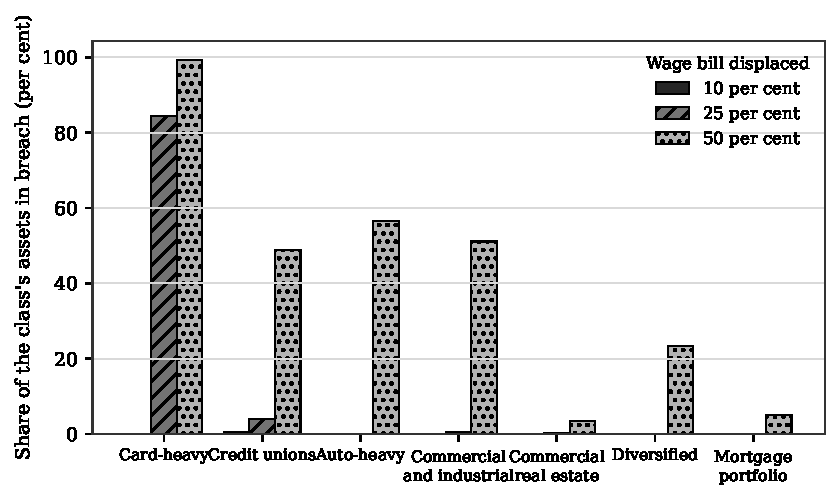
\includegraphics[width=0.84\textwidth]{fig5_breach.pdf}
\caption{Share of each business model's assets held by institutions below their capital threshold,
at three displacement levels. Balance sheets measured at 30 June 2026; loss application is
scenario, and the twenty-five and fifty percent levels are outside the observed data.}
\label{fig:breach}
\end{figure}

\subsection{The instrument test: household relief does not protect bank capital}

If the second round is what reaches banks, instruments acting on the first round should not do
much for bank capital. Table~\ref{tab:relief} tests that through the same balance sheets.
Forbearance, automatic income-driven student repayment and enhanced wage insurance together
remove \result{ReliefRemovedTen} percent of system bank losses at the ten percent level,
\result{ReliefRemovedTwentyFive} percent at twenty-five and \result{ReliefRemovedFifty} percent at
fifty: under a tenth everywhere. The arithmetic is in the first paragraph of this section, since
only \result{SysFirstTen} billion of a \result{SysLossTen} billion total is first round. The most
expensive instrument in the set costs \result{WageInsuranceCost} billion dollars and removes
\result{WageInsuranceRemoved} billion of bank losses.

\begin{table}[htbp]
\centering
\caption{Relief instruments against system bank losses at ten percent of the wage bill displaced.
Cells with no sourced fiscal cost read n/a. Scenario.}
\label{tab:relief}
\begin{tabular}{lrrr}
\toprule
Instrument & System loss removed (USD bn) & Per cent of system loss & Fiscal cost (USD bn) \\
\midrule
mortgage forbearance, partial & 2.60 & 1.27 & n/a \\
auto and consumer forbearance, partial & 5.35 & 2.61 & n/a \\
mortgage forbearance, full & 4.42 & 2.16 & n/a \\
auto and consumer forbearance, full & 9.10 & 4.44 & n/a \\
income-driven student repayment, automatic enrolment & 7.55 & 3.68 & 7.3 \\
wage insurance, current US, 0.50 for 26 weeks & 4.60 & 2.24 & 112.2 \\
wage insurance, enhanced, 0.70 for 52 weeks & 12.87 & 6.28 & 314.3 \\
All together: forbearance & 19.71 & 9.61 & 317.6 \\
\bottomrule
\end{tabular}

\end{table}

The conclusion is about what these instruments are for.

\begin{quote}
Household relief must be judged on household outcomes, not on bank capital. It does reshape the
distribution of failures: at the twenty-five percent level it takes assets in breach from
\result{ReliefAssetsBeforeTwentyFive} to \result{ReliefAssetsAfterTwentyFive} percent and stops
\result{ReliefStoppedTwentyFive} institutions breaching. It changes who fails, not how much is
lost.
\end{quote}

Those two facts are consistent. The instruments remove a small share of a large aggregate loss,
but they remove it from the institutions whose books are concentrated in the relieved categories,
so a small total with concentrated incidence changes many capital outcomes while barely moving the
system total. An instrument chosen to protect capital would have to act on the second round, which
means acting on spending, house prices and business credit.

\subsection{The exposures this engine does not reach}

Four sets of institutions are exposed in ways the panel does not capture, and naming them is more
useful than putting a number on them the data cannot support. \emph{State and local government} is
exposed through its own tax base, \result{StateLocalWageLinkedBn} billion dollars of wage-linked
income tax, \result{StateLocalWageLinkedShare} percent of its own tax receipts, and cannot run the
deficit through because of balanced-budget requirements; its in-year spending cut feeds the same
demand channel that produces nine tenths of the bank losses above, and that loop is not in the
engine, so its absence makes our figures conservative in a direction we can sign but not size.
\emph{Pension funds} are exposed on both sides at once, benefits fixed in nominal terms while
contributions are a share of covered payroll, so displacement widens the funding gap mechanically
and raises the required contribution rate on the employers who remain; the accounts capture only
the \result{PensionHoldingsBn} billion dollars they hold. \emph{Insurers and private credit} hold
both sides, insurers \result{InsurerHoldingsBn} billion dollars of wage-backed claims against
long-dated liabilities, while private credit cannot be separated from the other-financial
aggregate, so the \result{OtherFinancialHoldingsBn} billion attributed to that sector is an upper
bound by an unknown margin. And everything outside the insured depository system, nonbank
servicers and consumer lenders among them, is absent from the panel; as a class they are more
thinly capitalized than the institutions we measure, so the system figures are again a lower
bound.


\section{If AI fails}
\label{sec:bust}

The paper so far has asked what happens if AI succeeds and displaces labor. The opposite case
deserves the same treatment, and for most of this project it did not get it: displacement went
through a household engine, a fiscal module and thousands of balance sheets while the failure case
was assessed against historical analogies. That asymmetry flattered the failure case, so this
section runs it through the same machinery.

The answer is that an AI bust is a large fiscal event and a small credit event, which inverts the
displacement case exactly.

\subsection{What the AI side is financed with, in tiers}

Any claim about what a bust would do depends on how the investment was financed, so we set out
what is known in tiers, each with its own confidence label, and never blend them.
Table~\ref{tab:aitiers} gives them.

The hard tier is nine SEC registrants' own filings: \result{FilerCapexBn} billion dollars of
capital spending against \result{FilerOCFBn} billion of operating cash flow, a self-funding ratio
of \result{SelfFunding}, and \result{OnBalanceSheetAIDebtBn} billion dollars of on-balance-sheet
debt. On those books the debt-financed share of capital spending is
\result{DebtFinancedShare} percent. A second tier, verified from a Federal Reserve Bank source but
not from filings, is about \result{AIBankCommitmentsBn} billion dollars of large bank commitments
to AI-adjacent industries, of which roughly \result{AIDrawnBn} billion appears to be drawn. A third
tier, the equity value attributable to AI, has no defensible selection rule in our data and is
swept rather than asserted. The fourth tier, off-balance-sheet vehicles, GPU-backed lending, data
centre securitizations and vendor financing, is not sourced at all, and the Bank for International
Settlements describes exactly those structures as dominant in this market.

\begin{table}[htbp]
\centering
\caption{The AI side by tier of evidence. Tier 1 is measured from filings; tier 4 is the hole the
verdict turns on. Cells with no sourced value read n/a.}
\label{tab:aitiers}
\begin{tabular}{p{2.1cm}p{6.3cm}rp{3.1cm}}
\toprule
Tier & What it covers & Size (USD bn) & Confidence \\
\midrule
1 HARD & on-balance-sheet AI debt, nine named SEC filers & 458.4 & hard \\
2 VERIFIED SECONDARY & large bank C and I commitments to AI-adjacent industries & 450.0 & verified secondary \\
2b VERIFIED SECONDARY, drawn & the drawn share of those commitments, implied by the same source & 162.0 & implied from outstanding 9 pct vs committed 25 pct of tier 1 \\
3 SCENARIO & listed AI-exposed equity, swept share of US nonfinancial corporate equity & 7,200 to 21,598 & SCENARIO \\
4 NOT SOURCED & off-balance-sheet data centre vehicles, GPU-backed loans, private credit to data centres, data centre ABS and CMBS, vendor financing & n/a & NOT SOURCED \\
MEMO & chip supply chain & n/a & named \\
\bottomrule
\end{tabular}

\end{table}

\subsection{The verdict on the financing structure, which is conditional}

There are two historical patterns for an asset bust of this kind, and they have very different
fiscal consequences. In the equity-led case of 2000 to 2002, federal receipts fell
\result{EquityLedReceiptsPct} percent and corporate tax \result{EquityLedCorpPct} percent. In the
debt-led case of 2007 to 2009, receipts fell \result{CreditLedReceiptsPct} percent and corporate
tax \result{CreditLedCorpPct} percent. Both are verified from the published aggregates.

On the nine filers' own books, at \result{DebtFinancedShare} percent debt-financed, the structure
sits near the equity-led pattern. That is where a paper could stop, and it would be wrong to. The
verdict flips out of that pattern on \result{FlipToBetweenBn} billion dollars of additional
debt-financed capital spending, which is \result{FlipToBetweenShare} percent of the bank
commitments already identified in tier 2, and reaches the debt-led pattern on
\result{FlipToDebtLedBn} billion, \result{FlipToDebtLedShare} percent of them. The drawn portion of
those commitments alone is already larger than the first threshold. Tier 4 is unmeasured.

\begin{quote}
The defensible statement is that on the nine filers' own balance sheets the structure resembles the
equity-led case. The statement that the structure resembles the equity-led case is not defensible,
and we do not make it. The verdict is conditional on a quantity we have not measured, and the
direction of the unmeasured quantity is towards the worse case.
\end{quote}

\subsection{The bust run through the same engine}

Converted to a wage-bill equivalent, an AI bust costs \result{BustWageLow} to
\result{BustWageHigh} percent of the wage bill, which is \result{BustRatioLow} to
\result{BustRatioHigh} times smaller than the ten percent displacement case this paper has used
throughout. Household credit losses are \result{BustCreditLow} to \result{BustCreditHigh} billion
dollars, against tens of billions in the displacement case. Output falls \result{BustGDPLow} to
\result{BustGDPHigh} percent, well inside the fall in the Federal Reserve's severely adverse
scenario. All of these are scenario figures.

Federal receipts, on the other hand, fall \result{BustReceiptsLow} to \result{BustReceiptsHigh}
billion dollars on the verified historical episodes. That is an order of magnitude larger than the
terminal-year fiscal loss at ten percent displacement, and it arrives through a completely
different door: capital gains and corporate receipts rather than wage taxes.

Why the bust transmits so weakly to households is measured rather than assumed, and it is the same
ownership fact that drove Section~\ref{sec:fiscal}. Corporate equity is extraordinarily
concentrated: the top one percent of households hold \result{TopOnePctEquity} percent of it and the
bottom half hold \result{BottomHalfEquity} percent. A fall in equity value therefore lands on the
households with the lowest propensity to consume out of wealth, measured at \result{MPCWealth}
cents in the dollar per year. The same concentration that makes the capital tax base hard to reach
makes the wealth channel weak.

Two caveats belong with these numbers. The propensity to consume out of wealth is a sourced
parameter checked against two episodes, not a parameter we estimated. And the path through which
output falls does not feed bank-channel damage back into itself, so the output fall is understated
by an amount we have not sized.

\subsection{The payoff by holder, and what a holdings table cannot show}

Table~\ref{tab:payoff} scores each holder by its share of the wage side and its share of the AI
side, and reports the net position in three outcomes. Only the federal government and banks lose in
every column. Everyone else holds enough of the AI side to offset what they lose on the wage side
if AI succeeds: households in particular hold \result{HouseholdsAISide} percent of the AI side
against six percent of the wage side, and gain \result{HouseholdPayoffSuccess} under success where
the federal government loses \result{FedPayoffSuccess}.

\begin{table}[htbp]
\centering
\caption{The position of each holder across three outcomes, scored on holdings. The wage side is
measured; the AI side is scenario and a lower bound.}
\label{tab:payoff}
\begin{tabular}{lrrrrr}
\toprule
Holder & Wage side & AI side & AI fails & Partial & AI succeeds \\
\midrule
Federal government & 0.3215 & 0.0100 & -0.0132 & -0.1657 & -0.3115 \\
Banks & 0.1844 & 0.0318 & -0.0337 & -0.1081 & -0.1525 \\
Rest of the world & 0.1801 & 0.1808 & -0.1826 & -0.1804 & +0.0007 \\
Other financial & 0.1532 & 0.1633 & -0.1648 & -0.1583 & +0.0101 \\
Households & 0.0607 & 0.3842 & -0.3848 & -0.2224 & +0.3235 \\
State and local & 0.0462 & 0.0363 & -0.0367 & -0.0413 & -0.0100 \\
Insurers & 0.0203 & 0.0207 & -0.0209 & -0.0205 & +0.0003 \\
Unallocated remainder & 0.0164 & 0.0979 & -0.0981 & -0.0572 & +0.0816 \\
Pension funds & 0.0110 & 0.0437 & -0.0439 & -0.0274 & +0.0327 \\
Nonfinancial business & 0.0062 & 0.0313 & -0.0313 & -0.0187 & +0.0250 \\
\bottomrule
\end{tabular}

\end{table}

The table understates the federal position in the first column and the reason matters more than the
table. It scores holders by what they hold, so a government holding one percent of the AI side
scores as barely exposed when AI fails, at \result{FedPayoffFails}. But federal receipts fall
\result{BustReceiptsLow} to \result{BustReceiptsHigh} billion dollars in exactly that case. The
state's claim on the AI upside is fiscal rather than proprietary: it is the capital tax of
Section~\ref{sec:fiscal}, not a portfolio. A holdings table cannot see a tax claim, which is why
this paragraph sits beside the table rather than in a footnote.

Read that way, the two facts are one fact. Being barely exposed to an AI bust, in holdings terms,
and being unhedged on the AI upside are the same statement about a government whose only claim on
AI capital is a tax that reaches \result{TauKBarkai} percent of the surplus.

\subsection{Two directions, two tax bases}

The instruments that would protect against the two failure directions are nearly disjoint, but not
for the reason it would be natural to assume. It is not that a bust leaves the wage side untouched:
it touches it, and the size of that is reported above. It is that the bust reaches the wage side
through a channel one to two orders of magnitude smaller than displacement does, while reaching the
federal budget through capital gains and corporate receipts, which displacement barely touches.

The two failure directions therefore hit the same institution through different tax bases.
Instruments that protect the wage tax base do not protect the capital tax base, and the reverse.
That is the organising conclusion this paper carries into
Section~\ref{sec:institutions}: one capital tax rate is simultaneously the state's only claim on
the AI upside and the thing that would have to rise to close the fiscal condition after
displacement. It is being asked to do two opposite jobs.


\section{Institutions, by regime}
\label{sec:institutions}

This section draws out what follows from the measurements for institutions and for the people the
exposure ultimately reaches. It separates what the evidence supports from what it does not,
because recommendations are the easiest part of a paper of this kind to overreach.

\subsection{The organizing conclusion}

\begin{quote}
The federal government is fiscally exposed in both states, through different tax bases: wage taxes
if AI succeeds, capital gains and corporate taxes if it fails. Instruments that protect one base
do not protect the other.
\end{quote}

That is why the capital tax instrument is the only one that appears in both directions, and why
the contested base in Section~\ref{sec:fiscal} is the hinge rather than a technical footnote. The
rate links the two states without trading one against the other: as Section~\ref{sec:bust} shows,
bust-state revenue at risk is linear in the rate, so raising it scales both sides of the position
together, and the level cannot be sized without a measure of US AI capital income.

\subsection{What is needed at each regime}

For each regime we state the minimum instrument set identified by the measured mechanisms, which is a narrower claim than a policy recommendation. Appendix~\ref{app:detail} sets the four regimes and the failure case out in full. The shape of it is this. In the least-extrapolated scenario the set is the capital tax instrument, the trust fund contribution base, the student loan trigger and better measurement, and it is the only regime where we can say what is unnecessary as confidently as what is not: the housing agencies absorb that level without a Treasury draw and the banking system barely moves. At larger displacement nearly everything enters, with ownership and direct-claim instruments arriving precisely because the tax instrument is at its limit. Sudden displacement reorders the same set, since only contract instruments act inside a quarter, so pre-authorization is the whole instrument. At near-total displacement the required rate lies far outside observed experience and the question stops being financial regulation. In the failure case only concentration limits on AI-linked lending and the capital tax rate remain.


\subsection{What ownership would cost}

Because ownership is the instrument that survives at the extreme, its price is worth stating.
Raising the state's share of an AI side worth about \result{AISideTotalBn} billion dollars from
\result{AIFederalShareRounded} to ten percent would cost roughly \result{StakeForTenPctBn} billion
dollars and close about \result{GapClosedAtTenPct} percent of the gap, a stake about
\result{StakeVersusAgencyCapital} times the entire capital of the housing agencies. That is why
most instruments in Appendix~\ref{app:instruments} are not ownership instruments, and why the
ownership row cannot be dismissed: at near-total displacement it is the only row left, and the
cost of a position rises with the price of the asset.

\subsection{What each type of institution should change}

What each type of institution should change, tied to its measured exposure and paired with what the evidence does not support, is set out in Appendix~\ref{app:detail}.


\subsection{What the evidence does not support}

Two claims are tempting and neither survives the measurement: wholesale change to household mortgage underwriting at moderate displacement, and occupation-based underwriting. Appendix~\ref{app:detail} sets out the three measured grounds for the first and, for the second, the legal position, which is that occupation is not a prohibited basis under the Equal Credit Opportunity Act but that occupation-based underwriting in housing credit exposes a lender to a discriminatory-effects claim under the Fair Housing Act. Combined with the finding that the exposure is spread almost evenly across borrowers, the risk-adjusted case for it is weak and the case for portfolio-level disclosure is strong.


\subsection{Emerging markets}

Three facts change the answer outside a reserve-currency economy and they compound: imported AI capital accrues its taxable surplus abroad, a sovereign that cannot borrow in a currency it issues cannot absorb the shock, and many such economies are already on a steep debt path. The measurement itself is also unavailable there. Appendix~\ref{app:detail} gives the figures and the reason.


\subsection{State-contingent triggers}

Instruments are more useful attached to a trigger carrying its current value. The capital tax trigger is already tripped: the assembled rate is \result{TauKBarkai} percent against a threshold of \result{RequiredEasy} percent, both sides observed today. Prime-age nonemployment stands at \result{PrimeAgeNonemp} against the observed maximum of \result{PrimeAgeMax}, where the reemployment fit leaves the data, so crossing it is the moment the rest of this architecture can no longer be sized. Appendix~\ref{app:detail} gives the rest, and Appendix~\ref{app:instruments} the full instrument table.


\subsection{Implications for individuals, organisations and society}
\label{sec:implications}

Four consequences are worth stating plainly, because the exposure is ultimately borne by people.

\emph{For the people displacement reaches.} The thinnest buffers are one quintile up from the
bottom, among households carrying the commitments of those above them without the income to
service them through a gap in pay, so relief designed around the bottom quintile misses them, as
does relief designed around occupation. If displacement arrives through hiring that does not
happen, the private loss shifts onto people at the start of their working lives and becomes
invisible to the separations data most early-warning systems watch.

\emph{For managers.} Wage risk is a concentration to be governed rather than a credit category to
be underwritten: it is uneven in a way the aggregate hides, and it cannot be managed by tightening
household underwriting, because most of what arrives comes through the second round. The
governance question is whether an institution can state, in a form a board can read, how much of
its income and collateral depends on wages continuing to be paid, and what it has agreed in
advance to do if they are not.

\emph{Strategically.} Exposure to a fall in wage income sits on the federal balance sheet, and the
state's claim on the income that would replace those wages is the tax of
Section~\ref{sec:fiscal}, which falls short of what replacement needs. Acquiring a direct claim
instead is expensive, and a government that notices late will find the price of the asset has
risen for the same reason its revenue fell. An exposure spread almost evenly across the system
cannot be diversified away inside it, which makes pre-agreed rules and disclosure the instruments
with the best ratio of value to cost.

\emph{For society.} The claims wages pay are spread far more evenly than the wages themselves, so
a proportional fall in pay is regressive before any response is chosen. The same ownership
concentration runs through both halves of the paper: the capital tax reaches little because most
corporate claims sit where the income tax does not, and a bust transmits weakly because the assets
that would fall are held by the households least likely to change their spending. A statistic that
locates wage risk should be used to size public instruments, not to price individuals out of
credit for what they do for a living.


\section{Implications for individuals, organisations, and society}
\label{sec:implications}

The measurements in this paper are about balance sheets, but the exposure they describe is
ultimately borne by people, and the choices it forces are management and policy choices rather
than accounting ones. This section sets out what follows for four audiences.

\paragraph{For the people displacement reaches.} The household result that should travel furthest
is that the thinnest buffers are not at the bottom of the wage distribution. They are one quintile
up, among households that have taken on the commitments of the households above them without the
income or the assets to carry them: a median of \result{QTwoRunway} months of liquid runway, with
\result{QTwoUnderOne} percent holding less than a single month. A relief programme designed around
the bottom quintile misses them. So does a programme designed around occupation, because the
difference between physically and cognitively exposed households is almost entirely a difference
in pay, and what predicts whether a household survives a lost paycheque is what it earns rather
than what kind of work produced the earnings.

Two further findings bear directly on who carries the cost. If automation arrives through hiring
that does not happen rather than through layoffs, the private loss shifts onto people at the start
of their working lives, who hold student debt and little else, and it becomes invisible to the
separations data that most early-warning systems watch. And a claim that is serviced from wages is
a claim on somebody's pay: the reason this paper insists on the phrase \emph{labor backing} rather
than some more neutral term is that the aggregate is made of individual obligations that do not
adjust when the income behind them stops.

\paragraph{For managers and organisations.} The useful reframing for an institution is that wage
risk is not a credit category to be underwritten but a concentration to be governed. Three things
follow from the measured results. First, the exposure is uneven in a way the aggregate hides:
lenders whose books are unsecured consumer credit are the first to break and mortgage portfolio
lenders are among the last, which is close to the reverse of the intuition that housing is where
household risk lives. Second, an institution cannot protect itself against this exposure by
tightening household underwriting, because most of what reaches it arrives through the second
round, the spending and house prices and business credit that follow other people's lost wages,
and not through its own borrowers defaulting. Third, an institution that holds both sides of the
bet, insurers and private credit funds in particular, should report them together rather than in
separate parts of a disclosure, because the correlation between them is the whole point.

For a management reader the governance question is therefore not whether to buy a model of
automation risk. It is whether the institution can state, in a form a board can read, how much of
its income and how much of its collateral depends on wages continuing to be paid, and what it has
agreed in advance to do if they are not. Every contract instrument in this paper works only if it
was written before the event.

\paragraph{Strategic implications.} The strategic finding is about ownership, and it cuts against
the reflex to reach for a tax. The state holds the wage side of a two-sided bet and almost none of
the other side, and the only claim it has on the other side is a tax that reaches
\result{TauKBarkai} percent of the surplus against the \result{RequiredEasy} to
\result{RequiredHard} percent that replacing the lost wage taxes would need. Closing that position
by buying into the asset is priced in Section~\ref{sec:institutions} and it is expensive:
\result{StakeForTenPctBn} billion dollars to close about \result{GapClosedAtTenPct} percent of the
gap. Neither instrument is comfortable, and a government that notices this late will find that the
price of the asset has risen for the same reason its revenue fell.

The strategic reading for an organisation is parallel. An exposure that everyone holds cannot be
diversified away inside the system: our measurement is that it is spread almost evenly, so the
system in aggregate cannot rotate out of it even though any single institution can. That makes it
a candidate for pre-agreed rules rather than for portfolio management, and it makes disclosure the
instrument with the best ratio of value to cost.

\paragraph{For society and fiscal equity.} Three points are worth stating plainly. The first is
that the claims wages pay are spread far more evenly than the wages themselves, so a proportional
fall in pay is regressive before any policy response is chosen. The second is that the same
ownership concentration runs through both halves of this paper: the reason the capital tax reaches
so little is that most corporate claims are held in forms the individual income tax does not
reach, and the reason an AI bust transmits so weakly to household spending is that the assets that
would fall are held by the households least likely to change their spending. Concentrated
ownership makes the upside hard to tax and the downside narrow in its incidence, and those are the
same fact seen from two directions.

The third is about what a measurement like this is for. We deliberately do not use it to argue for
screening individual borrowers by occupation: Section~\ref{sec:institutions} sets out why the
evidence does not support it and why the legal exposure runs through discriminatory effects. A
statistic that identifies where wage risk sits should be used to size public instruments and to
make exposures visible, not to price individuals out of credit on the basis of what they do for a
living. That is a choice about how the measurement is used, and it belongs in the paper that
produces it.


\section{Limitations}
\label{sec:limitations}

Every limitation below is carried in the released limitations file and the numbering follows it.

\paragraph{L1. Off-balance-sheet and hardware-backed AI financing is unmeasured.} The AI side is
built from nine registrants' on-balance-sheet facts. Off-balance-sheet vehicles, which
\citet{BIS2026} identifies as dominant in data center financing, contribute nothing to it, and
neither does hardware-backed lending or securitization. Every level on that side is a lower bound
and every federal share of it an upper bound, which is why Sections~\ref{sec:aiside}
and~\ref{sec:bust} report it as bounds rather than as a point.

\paragraph{L2. Capital gains inside federal receipts are not separated.} The labor-linked share of
receipts splits the individual income tax by the wage share of adjusted gross income, and realized
gains sit inside that base, so the share overstates in years with large realizations and
understates in years without. The band is carried throughout and the federal exposure share moves
by under one percent across it; the fiscal magnitudes are more sensitive and we have not bounded
that.

\paragraph{L3. The novelty of the accounts is ``none located'', not ``none exists''.} No
systematic search with a stated protocol has been run for the specific question of whether anyone
has built this object before. The related-work audit did locate prior work on the fiscal
mechanism, and that priority claim was retired; the same could happen here.

\paragraph{L4. The holder split leaves an unidentified remainder.} Three of the four shares in the
mortgage holder split are read from a publisher and the fourth is an arithmetic remainder, treated
as private in full. That is conservative for our claim, since any federal fraction inside it would
raise the federal share, but we have not identified what is in it. A remainder of the same kind
appears on the AI side.

\paragraph{L5. The effective labor tax rate does not vary across the wage distribution.} It is a
single economy-wide rate. Because displacement is not uniform across the distribution, and the
incidence results show it concentrated away from the top, a flat rate probably overstates the
revenue loss from displacing low-paid workers and understates it from displacing high-paid ones.
We have not signed or bounded the net effect.

\paragraph{L14. The base of the taxable shareholder share decides how stable the capital tax
verdict is.} Ours is equity in taxable accounts over all US equity outstanding; the Congressional
Research Service uses the same numerator over domestically held stock alone. Ours is the right
base for a rate on a dollar of US surplus whoever holds it, but the choice is load-bearing: on the
other base the central rate rises to \result{TauKCRSCentral} percent, the share of the parameter
space that closes the condition rises to \result{TauKCRSPassShare} percent against the easier
labor tax reading, and the analytic maximum clears the harder threshold. The statement that no
corner of the space closes the condition holds only on our base and carries that qualification
wherever it appears; the center falls short on either base.

\paragraph{Method limitations.} Four are properties of the method. The \emph{extrapolation
boundary} of Section~\ref{sec:displacement}: above about a quarter of the wage bill displaced
there are no point estimates, only bands, which is a limit of the specification and not a fact
about the economy. The \emph{first-round scope} of the credit engine, which holds house prices,
spending, business revenue and the employment of everyone not displaced fixed, so every credit
loss is a floor. The \emph{procedural blind} in the rebuild protocol described in
Section~\ref{sec:rebuild}, which is why this paper says quantities were independently rebuilt
under a reported blind protocol and never that they were independently verified. And
\emph{foreign withholding}: dividends to foreign holders bear US withholding tax at treaty rates
and we treat them as untaxed at the owner level, which biases the assembled capital tax rate
downward by an amount we have not quantified, running against our own finding.

Five quantities that appeared in earlier versions of this work are not in this paper at all:
three because an independent rebuild could not reproduce them and our own specification was not
precise enough to show the rebuild wrong, one because the object it referred to was never defined,
and one because there is no such number to report. Appendix Table~\ref{tab:removed} lists each
with its reason.

\paragraph{Avenues for further work.} Each addresses a limitation above. Build the
off-balance-sheet side from securitization prospectuses, vehicle-level filings and supervisory data
on lending secured against computing hardware, so the AI side can be measured rather than bounded
(L1). Separate realized gains from wage income inside the individual income tax base and re-run
the fiscal magnitudes (L2). Run a systematic search with a published protocol for prior
constructions of a labor backing decomposition (L3). Identify the holder remainder from loan-level
sources (L4). Replace the single labor tax rate with rates by position in the income distribution
(L5). Construct both bases for the taxable-holder share from the same holder data and report the
rate on each (L14). Extend the reemployment relationship using a source that observes larger
displacement episodes, which would turn the bands above a quarter of the wage bill into estimates;
let house prices, spending and non-displaced employment move together, which would also let the
state and local feedback loop be modeled rather than named; run a rebuild with an enforced blind
and expected values held by a third party; and quantify withholding tax on dividends to foreign
holders, reporting the corrected rate even though it runs against our own finding.


\section{Conclusion}
\label{sec:conclusion}

The federal government is exposed, as holder, guarantor or debtor, on about
\result{SovereignUnion} percent of the claims paid directly from wages, and holds about
\result{AIFederalShareRounded} percent of the claims on AI capital; about
\result{DebtOnlyDirect} percent of all US debt, public and private, is serviced directly from
wages, government debt entering that measure through the labor-linked share of the receipts that
service it rather than because a household owes it, and the state stands behind most of it.
Displacement is a fiscal event before it is a financial one: at the one level fully inside the
observed data the federal government bears roughly four fifths of the first-round loss while the
banking system barely moves, and whether the budget absorbs that turns on which capital tax rate
reaches AI profits, since the condition needs \result{RequiredEasy} to \result{RequiredHard}
percent and the income that moves from wages to AI capital bears \result{TauKBarkai} percent once
every layer of tax is counted once. The state loses in both failure directions through different
tax bases, wage taxes if AI succeeds and capital gains and corporate taxes if it fails, so the
same capital tax rate is being asked to do two opposite jobs, and that, rather than any single
loss estimate, is what the measurement is for.

This paper is written for the people who will have to answer those questions with numbers: the
fiscal authority that has to decide whether to pre-fund, the supervisor that has to decide which
scenario to run, and the analyst who has to say how much of a balance sheet depends on wages
continuing to be paid. Everything reported here is generated from artifacts in a public
replication package, each carrying its status and its replication flag, so that a reader who
disagrees with a convention can change it and see what moves.


\section*{Declarations}

\ifanon
\paragraph{Data availability.} The replication package, including the measured artifacts behind
every reported value, will be made available upon acceptance.
\else
\paragraph{Disclosure statement.} The authors report no conflict of interest.
\paragraph{Funding.} This research received no external funding.
\paragraph{Data availability.} The replication package, including the measured artifacts behind
every reported value and the sealed expected values used in blind replication, is available from
the corresponding author.
\fi

\paragraph{Use of generative AI.} During the preparation of this manuscript the authors used a
generative AI tool to assist with language editing and refinement of the text. The authors
reviewed and edited all output and take full responsibility for the content of the paper. The
study's data were produced entirely by the measurement pipeline described in the paper, and no
reported value originates in a language model's assertion: every number in the text and in the
tables is generated from a measured artifact in the replication package. The tooling used to
build and to rebuild that pipeline is set out in Section~\ref{sec:data}.

\appendix

\section{The instrument table}
\label{app:instruments}

Table~\ref{tab:instruments} gives one row for each of the twelve instruments discussed in
Section~\ref{sec:institutions}: the institution that must act, the instrument itself, its type,
and the regime in which it binds. The table is generated from the released architecture file, and
that file carries the measured mechanism, the verified precedent and the trigger with its current
value for every row.

{\small\begin{tabular}{p{0.4cm}p{3.2cm}p{4.4cm}p{1.5cm}p{3.6cm}}
\toprule
\# & Institution that must act & Instrument & Type & Binds in \\
\midrule
1 & Tax authority (Congress, Treasury, IRS) & Narrow the gap between the AI-specific and economy-wide capital rates: limit expensing on labour-displacing assets, capture shifted rents, or tax the distribution rather  & tax & inside the data and larger displacement; fails at near-total displacement, see 4(d) \\
2 & Treasury, and the fiscal authority setting the debt path & Pre-fund or term out the labour-linked obligation stock while the labour tax base is intact & stock & all regimes; the only instrument that acts BEFORE the dose \\
3 & Treasury, or a statutory fund & Direct equity or revenue claim on AI capital: sovereign fund, golden share, or a public stake taken in exchange for public inputs & ownership & larger, sudden and near-total displacement; unnecessary inside the data \\
4 & Social insurance system (SSA, CMS, Congress) & Broaden the contribution base beyond covered wages, or convert to a general-revenue claim; and raise UI generosity and duration, which has a MEASURED effect on automation & flow & all regimes; binds SOONEST, because depletion arrives before any AI dose does \\
5 & Housing agencies (FHFA, Fannie, Freddie, FHA, Ginnie) & Forbearance and payment-deferral protocol pre-authorised for a displacement trigger; raise credit enhancement on the unenhanced book & contract & larger and sudden displacement; unnecessary inside the data, where no draw is triggered \\
6 & Student loan system (Education, servicers) & Income-driven repayment with an automatic displacement trigger; the claim already flexes with income & contract & all regimes, and it is the CHEAPEST row here because the instrument exists \\
7 & Auto lenders and ABS investors; supervisors for the bank-held slice & Displacement-contingent payment holiday in auto contracts; ABS documentation that anticipates it & contract & larger and sudden displacement \\
8 & Bank supervisors and the central bank & An automation scenario in the supervisory stress test, routed through spending, house prices and business credit, reported as a BAND & buffer & larger and sudden displacement \\
9 & Bank supervisors & Concentration limits or a supervisory add-on for AI-linked lending & buffer & the AI-fails case above all; also larger displacement \\
10 & Bank supervisors, statistical agencies & NOT wholesale mortgage underwriting change. Instead: disclosure of occupational exposure concentration at portfolio level & statistics & larger displacement only \\
11 & Statistical agencies (BLS, Census, BEA) & Measure reemployment, destination wages and never-hired entry directly and at higher frequency & statistics & all regimes; it is the precondition for every trigger below \\
12 & Emerging-market fiscal authorities; IMF surveillance & Source-based taxation of imported AI services; reserve and debt-path buffers built before the dose & tax & all regimes, and it binds HARDEST because the instruments above are unavailable \\
\bottomrule
\end{tabular}
}

\bibliographystyle{apalike}
\bibliography{references}

\end{document}
